\documentclass[11pt, oneside]{article}   	% use "amsart" instead of "article" for AMSLaTeX format
\usepackage[margin = 1.1in]{geometry}            		% See geometry.pdf to learn the layout options. There are lots.
\geometry{letterpaper}                   		% ... or a4paper or a5paper or ... 
\usepackage[parfill]{parskip}    		% Activate to begin paragraphs with an empty line rather than an indent
\usepackage{graphicx}				% Use pdf, png, jpg, or eps§ with pdflatex; use eps in DVI mode
								% TeX will automatically convert eps --> pdf in pdflatex	
\usepackage{adjustbox}	
\usepackage[section]{placeins}



%% LaTeX Preamble - Common packages
\usepackage[utf8]{inputenc}
\usepackage[english]{babel}
\usepackage{textcomp} % provide lots of new symbols
\usepackage{graphicx}  % Add graphics capabilities
\usepackage{flafter}  % Don't place floats before their definition
\usepackage{amsmath,amssymb}  % Better maths support & more symbols
\usepackage[backend=biber]{biblatex}
\usepackage{amsthm}
\usepackage{bm}  % Define \bm{} to use bold math fontsx
\usepackage[pdftex,bookmarks,colorlinks,breaklinks]{hyperref}  % PDF hyperlinks, with coloured links
\usepackage{memhfixc}  % remove conflict between the memoir class & hyperref
\usepackage{mathtools}
\usepackage[T1]{fontenc}
\usepackage[scaled]{beramono}
\usepackage{listings}
\usepackage{physics}
\usepackage{tensor}
\usepackage{tikz} 

\usepackage{helvet}

\newtheoremstyle{slanted}
  {\topsep}%   Space above
  {\topsep}%   Space below
  {\slshape}%  Body font
  {}%          Indent amount (empty = no indent, \parindent = para indent)
  {\bfseries}% Thm head font
  {.}%         Punctuation after thm head
  {0.5em}%     Space after thm head: " " = normal interword space;
     %         \newline = linebreak
  {}%          Thm head spec (can be left empty, meaning `normal')
  
%% Commands for typesetting theorems, claims and other things. 
\newtheorem{theorem}{Theorem}
\theoremstyle{slanted}
\newtheorem*{thm}{Theorem}

\newtheorem*{claim}{Claim}
\newtheorem*{example}{Example}
\newtheorem*{defn}{Definition}

\newcommand{\Lagr}{\mathcal{L}}
\newcommand{\vc}[1]{\mathbf{#1}}
\newcommand{\pdrv}[2]{\frac{\partial{#1}}{\partial{#2}}}
\newcommand{\thrint}[1]{\int d^3 \vc{x} \left( {#1} \right)}
\newcommand{\lalg}{ \mathcal{ G } } 
\newcommand{\rea}{ \mathbb{ R} } 
\newcommand{\com}{ \mathbb{ C} } 
\newcommand{\al}{ \alpha} 
\newcommand{\be}{\beta} 

\title{Part III Symmetries, Fields and Particles}
\author{Notes by Afiq Hatta, based on lectures by Nick Dorey and notes by Nicholas Manton}
\begin{document}
\maketitle
\tableofcontents

\pagebreak 

\section{What is a symmetry?}
Let's ask ourselves what is a symmetry? A symmetry is an operator we can do on variables (either dynamical variables or the coordinate frame or otherwise), which leaves physical laws invariant. This is completely analogous to the idea of spatial symmetries, where operators in space leave structures invariant. 

Let's analyse one of our most simple symmetries useful for physics - the rotation. We can motiavate what rotations look like based on how they act on vectors. A rotation would look like the map: 
\[ 
	\mathbf{v} \rightarrow \mathbf{v}' =  M \mathbf{v} 
\] 
But, we have extra restrictions on this. Firstly a rotation should preserve our length of vectors and hence our squared legnth $\mathbf{v}^T \mathbf{v} $. This means that 
\[ 
	\mathbf{v}'^T \mathbf{v}' = \mathbf{v}^T  M^T M \mathbf{v}  = \mathbf{v}^T \mathbf{v} 
\]
Which implies that $M^T M = I$. In addition, the orientation of vectors should be preserved, which means that we can't 'flip' vectors. This imposes the condition that $\det M = 1$.  
There's more reason to be had that $M^T M  =1$, owing to the fact that since physical laws are preserved, our Lagrangian should be preserved as well. 
This means that since our Lagrangian contains a kinetic term
\[ 
	\mathcal{L }  = \frac{1}{ 2} m \mathbf{v}^T \mathbf{v} + V( |\mathbf{x}|^2 ) \] 
we also have imposed the condition that $M^T M = I$, since this is the only way to make Lagrangians invariant. As a sanity check, physical laws of motion should transform under these rotations as well. This is trivial to check in the case of linear transforms (which includes rotations)
\[ 
	\mathbf{F}  = m \ddot{ \mathbf{x} } \implies \mathbf{F}' = m \ddot{x}  ' 
\]  
This result is achieved by just multiplying both sides by $M$. 

\subsection{Groups to represent symmetries}
Intuitively, symmetries should follow a group structure if we represent them as maps. For example, if we compose two symmetries together we should expect to obtain another symmetry. Similarly, we also expect symmetries to have inverses. This is where the notion of groups becomes useful for us. A group is a set $G$ with an operation $\_ \,  \cdot \,  \_ : G \times G  \rightarrow G $ which obeys the following axioms

\begin{itemize} 
	\item \textbf{Existence of a group identity }  $ \exists e \in G $ such that for all $g \in G$, multiplication satisfies 
	\[ e \cdot g = g \cdot e = g \] 
	\item \textbf{Existence of unique group inverses } for all $g \in G$we have a unique group inverse denoted $g^{ -1}$ such that 
\[ g^-1 \cdot g = g \cdot g^{ -1}  = e \] 
	\item \textbf{Associativity } this means that we don't care about the order in which we multiply things things in the group. So, for all $g_1, g_2, g_3 \in G$, we have that 
\[ 
	g_1 \cdot (g_2 \cdot g_3)  = (g_1 \cdot g_2 ) \cdot g_3 
\] 
\end{itemize} 
If the ordering of multiplication doesn't matter, in other words if, for all elements $g, h \, \in G$ we have 
\[ 
	g \cdot h  = h \cdot g 
\] 
then our group is called \textbf{Abelian}. Otherwise, it's called a non-abelian group. Our group of rotations is non-abelian, because the order in which you compose operations matters. For example, rotating something about the x-axis 90 degrees clockwise and then about the z-axis 90 degrees clockwise is different to rotating first about the z-axis, then rotating about the x-axis. 

In the case of rotations in three dimensions, we have a group which we'll call the special orthogonal group in three dimensions, or $S0(3) $. 
\subsection{Symmetries correspond to conserved quantities}  
Physics, the existence of symmetries lead to conserved quantities. In the case of rotations, in classical mechanics, rotational invariance leads to conservation of angular momentum by Noether's theorem. This is a conserved quantity derived from a symmetry acting on $\mathbb{R}^3 $. This manifests itself in the form of an angular momentum vector $\mathbf{L }  = (L_1, L_2, L_3 )$.  

In quantum mechanics, instead of phase space, we can work on Hilbert space $\mathcal{H}$, and do something similar. In Hilbert space, we work with state vectors $\ket{ \phi} \in \mathcal{H}$ and observable quantities are Hermitian operators $\hat{ \mathcal{ O }} $. Looking at generators of the rotation group, our analog of the angular momentum vector are angular momentum generators $\hat{ L}_i$ which we obey a 'spin' algebra 
\[
	 [\hat{L}_i, \hat{L}_j ] = i \epsilon_{ ijk} \mathcal{L}_k
\] 
which, we'll see later, that our commutator of operators in quantum mechanics is precisely our Lie algebra in the context of $\mathcal{ L }SO( 3)$. 

\pagebreak
  
\section{Manifolds and Tangent Spaces}

\subsection{Manifolds}

A manifold $\mathcal{M}$ is a shape which looks like a 'flat plane' from the perspective of a creature standing on it. This means that at every neighbourhood on this manifold there exists a homeomorphism (a continuous function whose inverse is also continuous) from the neighbourhood to a subset of $\mathbb{R}^n$ for some $n$. This $n$ is the dimension of the manifold. An easy example to wrap one's head around is a sphere, which is a two dimensional manifold. 

More specifically, at every point $p \in \mathcal{M}$ there exists an open set $\mathcal{P} $ with a homeomorphism $\phi_p : \mathcal{ P } \rightarrow U \subset \mathbb{R}^n $. These maps are called coordinate charts, and our collection of open sets $\mathcal{ P}_i $ should cover the manifold. 
\begin{figure}[h]
	\centering 
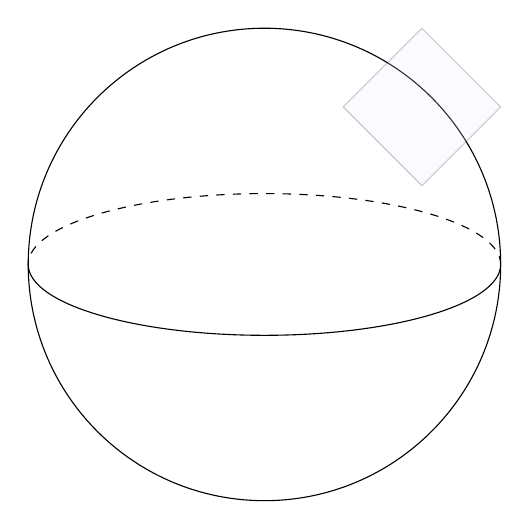
\begin{tikzpicture}
	\draw (0, 0) circle (3cm);
	\draw (-3, 0) arc (180:360:3 and 0.9);
	\draw[dashed] (3, 0) arc (0:180:3 and 0.9);

	\filldraw[fill=blue!10, opacity=0.2] (1, 2) -- (2, 3) -- (3, 2) -- (2, 1) -- cycle;  
   
\end{tikzpicture}
	\caption{A sphere locally looks like a flat plane, at any given point on the surface} 
\end{figure}

Since these homeomorphisms are from the manifold to $\mathbb{R}^n$, we can identify coordinates on an open set $\mathcal{P} \subset \mathcal{M}$, denoted by $\{ \theta^i \}$, where $i$ ranges from $i  = 1, 2, \dots, n$, where $n$ is the dimension of the manifold.

\subsection{Functions on manifolds} 
On this manifold, we can define objects like curves and scalar functions.  A function on a manifold is like a 'heatmap', 
\[
	f : \mathcal{M} \rightarrow \mathbb{R}. 
\]
This map $f$ can be smooth or not, of course. How do we define concepts like differentiability and continuity on functions on a manifold? Well, since the space is homeomorphic to $\mathbb{R}^n$, we can say a function $f : \mathcal{M} \rightarrow \mathbb{R}$ is differentiable provided that that its corresponding function $f' : \mathcal{U} \rightarrow \mathbb{R}^n$ is differentiable, where $U$ is the image of the homeomorphism from $\mathcal{M} \rightarrow \mathbb{R}^n$. 

Similarly, we can define curves on this manifold. Think of a path an ant takes on this curved space. A curve $\lambda$ is precisely this kind of path. This is a smooth map from an interval $I$, which without loss of generality we set $I = (0, 1)$, to the manifold. 
\[ 
	\lambda : I \rightarrow \mathcal{M}. 
\]

\subsection{Tangent vectors}
If we compose a curve with a function on a manifold, we get a function from $I \rightarrow \mathbb{R}$. This of this composition as taking a 'slice' of the function along the manifold. What interests us is that we can then take the derivative at $x = 0$ along this curve. 
Think of 
\[
	\frac{d f (\lambda (t))}{dt}\mid_{t = 0}, 
\]
which makes sense since $f \circ \lambda : I \rightarrow \mathbb{R}$. So, we're not doing anything suspicious here. 
This action of taking a function on a manifold and then differentiating it is interesting. With every curve, we can associate a differential operator which corresponds to differentiating a function on that curve. 

\subsection{Embedding manifolds in $\mathbb{R}^n$} 
Let's think about the manifold $S^2$. We've already defined an appropriate coordinate chart in this object, but a natural way to think about this surface is also to parametrise this as a surface in $\mathbb{R}^3 $, as a sphere with unit radius $1$. So, we're taking a manifold $\mathcal{M}$ and then finding a way to express this in some higher dimensional $\mathbb{R}^k$ (this is called an embedding).  We have that clearly
\[ 	
	S^2 = \{ \mathbf{x} \in \mathbb{R}^3 \mid |\mathbf{x}|^2  =1 \} 
\] 
Note that here, the way we parametrise $S^2$ is by specifying an element in $\mathbb{R}^n$ and then imposing a condition on the surface. More generally, we can embed a general manifold in $\mathbb{R}^n$ by writing it as 
\[ 
	\mathcal{M} = \{ \mathbf{x} \in \mathbb{R}^n \mid F_\alpha(\mathbf{x} ) = 0 \}  \]
where we have $l$ constraints given by $\alpha = 1, 2 \dots, l$, where $F_\alpha : \mathbb{ R}^n \rightarrow \mathbb{R}$, and is a smooth function. In the case of $S^2$, we have that $\alpha = 1$, and 
\[ 
	F_1 ( \mathbf{x} ) = |\mathbf{x}|^2 - 1
\]  
\subsubsection{The Embedding Theorem} 
A natural question to ask ourselves is how we can relate our dimension of our manifold to the dimension of our embedded space and our number of constraints. This is where the embedding theorem comes in. If we have $\alpha = 1, 2 \dots, l$, then the dimension of our manifold $\mathcal{M}$ is of dimension $m  - l$, where $m$ is the dimension of the space we're embedding in, if and only if 
\[ 
	J\indices{^\alpha_\beta} = \frac{ \partial F_\alpha}{ \partial x^ \beta} \] 
is of full rank $l$ everywhere on our manifold.
In the case of our 2-sphere, we had that in components 
\[ 
	F(x, y, z) = x^2 + y^2 + z^2 - 1 \implies J = 2( x, y , z) 
\] 
But in this case, on the manifold, $(x, y, z) \neq ( 0 , 0 , 0)$, so is of rank $1 = l$ everywhere. Hence the dimension of $S^2$ is $3 - 1 = 2$. 
 
\subsection{Classifying manifolds} 
We can classify manifolds by some of their topological properties. We'll outline them here. 

\begin{itemize} 
	\item Connectedness is the property that we can construct a path from anywhere in the manifold to any other point in the manifold. For example, a sphere is connected, but a manifold whose set of points is two spheres is not. 
	\item Simply connectedness is subtly different from connectedness. It comes from the concept of a homotopy group. For a space to be simply connected, it means that any loop on the surface can be continuously deformed to a point. In the language of algebraic topology, we require that 
\[ 	
	\pi_1 ( \mathcal{M} ) \simeq \{ e \} 
\] 
Somthing that's not simply connected is a solid torus; since we can 'tie a string' around the centre donut. 
 	\item Compactness is when we can cover a space with a finite amount of subsets. This condition is equivalent to the condition, that if we're embedding in $\mathbb{R}^n$, then the subset is closed and bounded. 
For example, a quadratic curve on $\mathbb{R}$ is not a compact manifold since it's not bounded. 
\end{itemize}
 

\pagebreak
\section{Lie Groups}

\subsection{What is a Lie Group?}
A Lie group is a group of continuous transformations, which depends smoothly on $n$ given parameters, say. Since it takes $n$ parameters to define a transformation in this group, we could also interpret this as an $n$ dimensional manifold. Thus, we define a Lie group as a group which is also a smooth manifold. Thus, multiplication between group elements: 
\[ 
	G \times G \rightarrow G
\]
must respect the manifold's structure and must be a smooth map. In addition, inverses of elements must also be smooth maps. 
Since an n dimensional Lie group is homeomorphic around $e$ to an open subset of $R^n$, we can re-parametrize the elements of the group $G$ to depend on $n$ different coordinates, say $\{ \theta_i \mid i = 1, \dots, n\} $. 

Let's have an example of maps which respect group structure. On a Lie group (or equivalently, a manifold), we can construct a 'left action' induced by an element $g \in G$, which in the context of a Lie group is simply multiplicaiton by that element on the left 
\[ 
	L_g: \, G \rightarrow G, \quad h \in G \mapsto gh \in G 
\] 
However, in the context of viewing a Lie group as a manifold, this map represents 'translating' a member $g$ on a manifold to it's new place. It turns out, that due to this translation map we've defined above, we can actually characterise most of our Lie group based on what happens infinitesimally at $e \in G$. We'll go over this later, but infinitesimal behavour at defines a tangent space which we call a \textbf{Lie algebra}. This notion is useful because Lie groups and manifolds are complicated, but defining the tangent space is handy because it's a \textbf{vector space}. This tangent space, you guessed it, is exactly what we've defined abpve.  

\subsubsection*{Smoothness of group multiplication on manifolds} 
Our condition that group multiplication and inversion should be smooth maps on the manifold is a statement about smoothness of coordinate maps. Since we can define a coordinate chart on an open set in the manifold, we can denote group elements $g \in G$ by their coordinates. So, we can write 
\[ 
	g  = g (\theta) \in G 
\] 
where $\theta  = ( \theta_1 , \dots, \theta_n)$, and our identity $e \in G$ lies at $g ( 0 )$. 
Group multiplication in $G$ is a map 
\[ 
	G \times G \rightarrow G, \quad g \times g' \mapsto g''  
\] but since we can assign coordinates to elements in a Lie group, we can write this multiplication as 
\[  
	g(\theta) \times g(\theta') \rightarrow g(\theta'') 
\] 
where we assume that $\theta''$ lies in the image of the same coordinate path $\mathcal{P}$ that we used to assign coordinates to $\theta, \theta' $. This implies that we've induced a map between coordinates on the manifold, and we express the function $\theta''$ as a function of the other coordinates. 
\[ 
	\theta''  = \theta''( \theta, \theta' )
\] 
Thus, one of the conditions for a group to be a Lie group is that this induced map $\mathbb{R}^n \times \mathbb{R}^n \rightarrow \mathbb{R}^n $ must be smooth (differentiable). More specifically, each of the components of this function $(\theta'')^i  = (\theta'')^i ( \theta, \theta' ) $ must be smooth. 

\subsubsection*{Smoothness of inversion of Lie Groups} 
In a group, taking an inverse is the operation 
\[ 	
	G \rightarrow G, \quad g \mapsto g^{ -1} \text{ where we have } g g^{ -1}  = e
\] 
Just as in the case of group multiplication, we can write in terms of coordinates on our manifold where we have 
\[ 
	g(\theta) \rightarrow g(\hat{\theta})  = (g(\theta))^{-1} 
\] 
This induces a map between coorinates 
\[ 
	\theta \mapsto \hat{ \theta} 
\] Our condition that this group is a Lie group is that this operation between coordinates is also differentiable. 

As an example, the additive group of vectors on $\mathbb{R}^d$, denoted $( \mathbb{R}^d, + )$, is a lie group. Group operations on this space between vectors are 
\begin{itemize} 
	\item Addition: $\mathbf{x}_1  + \mathbf{x}_2 = \mathbf{x}_3 $ 
	\item Inversion: $\mathbf{x} \mapsto  - \mathbf{x} $
\end{itemize} 
The corresponding coordinates are just their Euclidean coordinates $\mathbf{x} = (x_1, \dots, x_n ) $, and addition is represented by the usual way to add coordinates in $\mathbb{R}^n$, which is obviously continuous and differentiable. In addition, inversion is just attaching a minus sign to map $(x_1, \dots, x_n ) \mapsto  - ( x_1, \dots, x_n ) $, which is also a smooth map. 


\subsubsection*{A remark on classifying Lie algebras}

It turns out, we can classify all finite semi-simple Lie algebras over $\mathbb{C}$. into four infinite families denoted $A_n, B_n, C_n, D_n$, where $n \in \mathbb{N}$ with five exceptional cases: Lie algebras denoted $E_6, E_7, E_8, G_2$ and $G_4$. This is called the Cartan classification for Lie algebras and we'll cover it further later.  

\subsection{Matrix groups}
Given some field $F$, which could be either $\mathbb{C}$ or $\mathbb{R}$, we define the set of $n \times n$ matrices over it as $Mat_n (F)$. Let's choose matrix multiplication as our group operation. Clearly, there exists a mutliplicative identity, the identity map, and we also have by the definition of matrix multiplication that its associative. However, this set doesn't form a group in it's own right since not all matrices are invertible. However, we can pick out the set of invertible matrices 
\[
	GL_n(F) = \{A \in Mat_n(F) \mid det A \neq 0 \}  
\]
which we refer to as the general linear group. In fact, $GL(n, F)$ is a lie group in its own right, because matrix multiplication and inversion is smooth. We will also prove shortly that $GL(n, F)$ is an open set of $Mat_n(F)$, so our coordinate chart into $\mathbb{R}^{n^2}$ is just the identity map, and hence we have an $n^2$ dimensional Lie group.  

The special linear group is $SL_n(F)$ where our matrices have determinant 1, so 
\[ 
	SL(n, F) = \{ M \in GL(n, F) \mid det M = 1 \} 
\] 
This is a group by the multiplicative property of determinants where 
\[ 
	det(M_1 M_2) = det(M_1)det(M_2)
\] Hence, multiplying two matrices with determinant 1 also gives a matrix with determinant 1. We now ask ourselves what is the dimension of this Lie group? Well, we've embedded this object in as 
\[
	SL(n, F) = \{ M \in Mat_n(\mathbb{ R}) \simeq \mathbb{R}^{ n^2 } \mid det M = 1 \}
\]
Thus, if we can show that the function $F(M) = det M - 1 $ has a non-negative Jacobian at each point on the manifold, then we have an $n^2 - 1$ dimensional Lie group.  
We reindex the variables to differentiate with as $M_{ij}$. This looks weird but we're merely reindexing each component of the matrix in the completely natural way. Our Jacobian element (due to a result which we will not prove), is 
\[ 
	J_{ij}  = \frac{\partial F}{\partial M{ij} } = \pm det ( \hat{M}^{ ij } ) 
\] 
$\hat{M}^{ ij} $ represents the matrix of minors, which is the $(n - 1) \times ( n - 1) $ matrix that we get when we remove the $i$th row and $j$th column. It's a result that $det(\hat{M}^{ ij } )  = 0 \iff det(M) = 0, \quad \forall i, j = 1, 2,\dots n$, hence this $J$ is non zero and hence is of rank one. Thus, the dimension of our manifold is $n^2 -1 $. Furthermore, matrix multiplication and matrix inversion are smooth maps, hence this is a lie group. 

We can extend this argument to complex matrices where our condition that our determinant be 1 gives two constraint functions, since we're fixing a condition on both real and imaginary components. We have 
\begin{align*} 
dim (GL(n, \mathbb{R} ) &= n^2 \\
dim (SL(n, \mathbb{R} ) &= n^2 - 1\\
dim (GL(n, \mathbb{C} ) &= 2n^2 \\
dim (SL(n, \mathbb{C} ) &= 2n^2 - 2
\end{align*} 

\subsubsection{Matrix groups in $GL(n, \mathbb{R} )$} 
Our first matrix group that we'd like to examine is the matrix group whose action on vectors leaves their lengths unchanged.
\[ 
\mathbf{v} \mapsto \mathbf{v}' = M \mathbf{v} 
\] 
The condition that these maps leave lengths unchanged means that 
\[ 
|\mathbf{v}'|^2 = \mathbf{v}^T M^TM \mathbf{v}  = \mathbf{v}^T \mathbf{v} 
\] 
This implies that our matrix $M$ has to satisfy the condition that $M^M  = I$. This motivates the definition of the orthogonal group 
\[ 
O(n)  = \{ M \in Mat_n(F) \mid M^T M = I \} 
\] 
Taking determinants, 
\[ 
M^T M = I \implies det (M )^2 = 1 \implies det M  = \pm 1 
\] 
$O(n)$ defines a manifold since there's as chart to a subset of $\mathbb{R}^{n^2 } $ (although we don't know what dimension it is yet), but we can see that immediately that it's not a connected manifold. This is because of the fact that $det (M ) = \pm 1$ Taking a determinant is a smooth function of $M$, but there's no smooth path we can parametrise $M$ with on the manifold to swith the determinant from $+1$ to $-1$. This is becasue if there was, the composition of two smooth functions would be discontinuous, a contradiction.

So, we've essentially split $O(n)$ into two portions. If we focus on the part of the group where $det M  =1$, this gives us the special orthogonal group. 
\[ 
SO( n) = \{ M \in O(n) \mid det M  = 1\} 
\] 
This has the property that we're preserving the orientation of a basis of $\mathbb{R}^n $ say. Suppose we had a basis 
\[ 
\mathcal{B}   = \{ \mathbf{v}^1 , \dots \mathbf{v}^n \} 
\] 
Then a linear map is orentation preserving if the sign of 
\[ 
\Omega  = \epsilon^{ i_1 i_2, \cdots i_n} v^1_{i_1} \dots v^n_{i_n } 
\] 
is preserved after transformation of the vectors. Matrices with determinant 1 preserve the sign of this object. Hence $M \in SO ( n) $ are considered as rotations, where as matrices in $O ( n ) $ without unit determinant are considered some composition of rotations and reflections. 

The condition that $M^T M = I$ provides constraints only up to a transpose. This means that our constraints which are linearly independent only lie in the top triangle, which gives us $\frac{1}{ 2} ( n ) ( n + 1 ) $ constraints on our manifold. This means that, using the embedding theorem, 
\[ 
dim ( O (n) ) = n^2  - \frac{1}{2} ( n ) ( n + 1 )  = \frac{1}{2}( n )( n - 1) 
\] 
Since our condition already fixes that that $ det M  = \pm 1 $ up to a sign, this imposes no additional contraints on our manifold and we have that 
$dim SO( n )  = dim O(n)$. 

Matrix groups are Lie groups - the can parametrise them through their matrix entries smoothly, where each matrix element is a coordinate. With this reasoning, the dimension of $GL_n(\mathbb{R})$ is $n^2$, for example. 

\subsubsection{General properties of $O(n)$ } 
In this section, we'll look at some properties of some common orthogonal groups that will arise. To help us with this, we'll present some details about matrices in $ O (n) $ to help us with our discussion. In particular, facts about eigenvectors and eigenvalues, which are basis invariant properties, are particularly useful for our discussion. 

\begin{thm}

If $\lambda \in \mathbb{C}$ is an eigenvalue of $M \in O (n) $, then so is $\lambda^* \in C$ Furthermore, we have that $|\lambda|^ 2 = 1$. 
\begin{proof} 
Suppose that $\lambda \in C$ is an eigenvalue. Then by definition, there exists a (complex) vector $\mathbf{v} \in \mathbb{ C}^n $such that $M \mathbf{v}_\lambda = \lambda \mathbf{v}_\lambda $. However, recall that $M \in GL ( n , \mathbb{ R})$. This means we can take the complex conjugate (not transpose!) of this equation, and since the entries of $M$ are real, it doesn't change. This gives us 
\[ 
M \mathbf{v}_\lambda^* = \lambda^* \mathbf{v}_\lambda^* 
\] However, this implies that $ \mathbf{v}_\lambda^*$ is an eigenvector with eigenvalue $\lambda^*$. So we're done. Another way to phrase this is that since the entries of $M $ are real, then the coefficients of its characteristic polynomial are real. However, this means that any complex root must have it's complex conjugate as a root as well. 

We can use the orthogonality property to our advantage here. Note that 
\[
	|\mathbf{v}|^2 = \mathbf{v}^\dagger I \mathbf{v} = \mathbf{v}^\dagger M^T M \mathbf{v} = |\lambda|^2 |\mathbf{v}|^2 \implies |\lambda|^2  = 1
\] 
\end{proof}
\end{thm} 
This fact is important, this means that if we have a complex eigenvalue, then it must be a phase of the form $e^{ i \theta} $ and $e^{  - i \theta} $ must also be an eigenvalue. Our condition that modulus squared also applies to real numbers. If we have $\lambda \in \mathbb{ R}$, then $\lambda \in \{ -1, + 1 \}$. However, these are also phases and so are included in the condition above. 

\subsubsection{SO(2)} 
Take the group $SO(2)$. This is the matrix group 
\[ 
	SO(2) = \{A \in O ( n )  \mid \det A = 1 \}  
\] We have from our previous discussion that matrices in $O (n ) $ have eigenvalues which must be $e^{ i \theta}, e^{. -i \theta} $, with $\theta \in \mathbb{R}$. However, phases are invariant by shifting $\theta \rightarrow \theta + 2 \pi$, so we have the identification that 
\[ 
	\theta \sim \theta + 2 \pi 
\] This is suggestive that elements in the group represent rotations in the 2 dimensional plane. We can thus use $\theta$ as a coordinate to parametrise our manifold as rotations in the plane as $M(\theta)$, with a general group element written as 
\[ 
	g(\theta)  = \begin{pmatrix}
	\cos \theta &   - \sin \theta \\
	\sin \theta & \cos \theta
	\end{pmatrix}, 
\]
where we restrict $\theta \in S^1$. Thus, our corresponding manifold for this Lie group is the circle $S^1$, and $\mathcal{M} (SO(2)) \simeq S^1$. 
To reaffirm our confidence that this is a Lie group, one can check that $M ( \theta_1 ) M(\theta_2 )  = M(\theta_2)M(\theta_1) = M(\theta_1 + \theta_2) $, so group multiplication acts smoothly on the manifold. Furthermore, this manifold is connected, but not simply connected because tying a string around a circle, we can't contract this down to a point. In fact the homotopy group of $S^1$ is 
\[ 
	\pi_1 (S^1 ) \simeq \mathbb{Z}
\] This is because we can loop a string around $S^1 $ n times in an additive sense. 



\subsubsection{SO(3)}
We increase the dimension a bit and explore what's going on with $SO(3)$.Before we go into the maths behind representing rotations in three dimensions, let's first go into some of the geometrical intuition. To rotate something in three dimensions, a systematic way one could go about doing this is to first choose an axis of rotation which we could parametrise as a unit vector $\hat{\mathbf{n}} \in S^2 $ on our two-sphere. We can then rotate this. Naively, we'll say that we can rotate this by an angle $\theta \in [0, 2\pi)$, but more careful consideration tells us that if we parametrise rotations in this range, we're double counting. Rotating about the $\hat{ \mathbf{z} } $ axis by an angle of $ \theta  = \frac{ \pi }{ 2 } $ is exactly the same as rotating about the $ - \hat{ \mathbf { z} } $ axis by an angle of $ \theta  = \frac{ 3 \pi}{ 2} $. So, we have a \textbf{redundancy} in our initial idea of the range of $\theta \in [0, 2 \pi)$, and it's sufficient to parametrise elements in SO(3) with 
\[ 
	\hat{ \mathbf{ n } } \in S^2, \quad \theta \in [0 , \pi ) 
\] Now we can go into more detail about representing objects in SO(3) as matrices.  We first ask what our eigenvalues look like. Since the matrix elements of a matrix in $SO(3)$ are real, its characteristic polynomial has real coefficients. Thus, we must have one real eigenvalue and two complex eigenvalues. Due to the conditions we described earlier about orthogonal matrices, they eigenvalues are $1, e^{i \theta}, e^{ - i \theta}$. 
Given that $\mathbf{n}$ is a unit modulus eigenvector of $M \in SO(3)$ with $M \mathbf{n} = \mathbf{n}$, a general element in this matrix can be written as 
\[
	M(\theta, \mathbf{n}) = \cos \theta \delta_{ij} + (1 - \cos \theta) n_i n _j  + \sin \theta \epsilon_{ijk} n_k. 
\]
We're interpreting $\mathbf{n}$ to be the axis of rotation, since it's an invariant vector. Notice that there's some ambiguity in our description here. For example, if we were to map $\theta \rightarrow 2 \pi - \theta$, this gives us the same result as if were to map $\mathbf{n} \rightarrow - \mathbf{n}$, which we argued in the previous paragraph\. . In addition, rotating about a given axis by 0 degrees does nothing, so we have even more redundancy in this system. We have the following identifications on our manifold $M$: 
\[ 
	M( - \mathbf{n}, \theta ) \sim M ( \mathbf{n}, 2\pi - \theta), \quad M(\mathbf{n}, 0 )  = I_3, \quad \theta \in [ 0, \pi] 
\] 
Now let's ask ourselves, what are problematic values of $\theta$ and where can we identify what things with what things? Well, since we require that 
\[ 
	\theta \in [0,\pi ], 2 \pi  -\theta \in [ 0, \pi ] \implies \pi \leq \theta \leq 2 \pi \implies \theta = \pi 
\] is where our things need to be identified. So, we have the identification that 
\[ 
	( - \mathbf{n}, \pi) \sim (\mathbf{n}, \pi )
\]  
Let's think of this geometrically by defining a new mapping from our manifold to a ball. Let's now parametrise the manifold in terms of a vector 
\[ 
 	\mathbf{w} = \theta \hat{ \mathbf{ n} }, \quad \theta \in [0, \pi ) 
\] This is already consistent with our second identification since when  $\theta = 0$, $\mathbf{ w}  = 0 $, an identity element. Now, it takes some work to wrangle this in a manifold that's compatible with the first identification structure. 
We can define the ball with radius $ \pi$. 
\[
	B_3  = \{\mathbf{w} \in \mathbb{R}^3 \mid |\mathbf{w}|^2 \leq \pi  \} 
\]
and its corresponding boundary 
\[
	\partial B_3 = \{\mathbf{w} \in \mathbb{R}^3 \mid |\mathbf{w}|^2 =\pi  \}. 
\] However, because of our identification condition earlier, we have that antipodal points on this boundary sphere are considered to be 'identified' or 'the same' with one another. So in actual fact, the boundary of this manifold is $\partial B_3  / \sim$, where our equivalence relation quotients our antipodal points. This means that our manifold has no boundary since points on the boundary sphere aren't unique. It's easy to see that whilst this manifold is connected, it's not simply connected because we can take a straight line going through the origin through the sphere, but since antipodal points are identified, this constitutes a loop. We can't contract this however since rotating this line will always keep us on the boundary. On the other hand, we can easily construct a loop just in the interior of this sphere. 

However, we can 'square' a loop by going straight through the sphere twice, and that curve \text{is} deformable to a point! This suggests that our homotopy group structure is akin to $\mathbb{Z}_2$, so 
\[ 
	\pi_1 ( SO ( 3) ) \simeq \mathbb{Z}_ 2 \simeq \{ +1, - 1 \} 
\] 
This manifold is compact since it's bounded, and closed since we're including points on the boundary. 

\pagebreak 
\subsubsection{Non compact groups; the Lorentz group and more general metrics}

We brought up orthogonal groups previously because they preserve the Euclidean metric
\[ 
	M^T M  = M^T I M. = I 
\] 
 However, there are matrices which preserve more general metrics, ubiquitous in physics. A metric with signature $(p, q)$, is of the form 
\[
	\eta = \begin{pmatrix}
		I_p & 0 \\
		0 & - I_q \\
	\end{pmatrix}. 
\]
We denote the matrices which preserve this metric as 
\[
	O(p, q) = \{ M \in Mat_n(F) | M^T \eta M = \eta  \} . 
\]
These are matrices which constitute the general orthogonal group. Our simplest example of a matrix in the class of general orthogonal matrices is the a general matrix in $SO(1,1)$, which looks strikingly similar to a rotation matrix in $SO(2)$, expect that we've replaced our sin and cos terms with 
\[ 	
	M  = \begin{pmatrix} 
		\cosh \phi & \sinh \phi \\
		\sinh \phi & \cosh \phi 
	\end{pmatrix}, \quad \phi \in \mathbb{R} 
\] 
One can easily check that this has determinant 1, and that it preserves the metric $diag ( 1, - 1)$ However, since our coordinate parameter $\phi \in \mathbb{R} $, this group is not compact since $\mathbb{R}$ is not compact. 


\subsubsection{Subgroups of $GL(n, \mathbb{ C}) $}

Thus far, we've invested quite a bit of effort in looking at real matrices which have the interpretation of leaving vector norms unchanged. We can do the exact same with complex matrices. These matrices are analog of orthogonal matrices but in complex space instead, for $F = \mathbb{C}$. The set of matrices in this matrix group which leave the norm of complex vectors unchanged are the unitary matrices. 
\[
	U(n) = \{ M \in Mat_n (\mathbb{C}) \mid M^{\dagger} M = I \}. 
\] In analog with what we had in the real case, 
\[ 	
	\mathbf{v}' \in \mathbb{C}^n \mapsto \mathbf{v}' = M\mathbf{ v}, \implies  |\mathbf{v}'|^2 = |\mathbf{v}|^2 
\] Our condition for unitary implies that the determinant of matrices in the group is a phase, since 
\[ 
	| det ( M ) |^2 = 1 \implies det ( M) = e^{ i \theta}, \quad M \in U ( n) 
\] Our key difference that we have from the real case with $O(n)$ is now that we no longer have discontinuous jumps when taking the determinant, since our determinants vary by a smooth phase! This means that $U( n)$ is a connected manifold! Just as before, we can restrict our matrices in $U( n )$ to those which have unit determinant, 
\[ 
	SU ( n ) = \{ M \in U ( n ) \mid det M = 1\} 
\] 
By arguments that matrix multiplication in complex space is smooth, we have that $U ( n)$ and $SU ( n) $ are Lie groups. Thus, we can count their dimensions. If we consider complex numbers as being parameterised by 2 real numbers, our over-arching embedding space is $\mathbf{R}^{ n^2 } $. To figure out the dimension of $U (n)$, we need to impose the condition that 
\[ 
	 H = M^\dagger M  = I, \text{ equivalently } H^\dagger = H 
\]  On the surface this looks like we have $2 n^2 $ constraints, but this is symmetric up to hermitian conjugation. Hence, we ask how many degrees of freedom we need to define a Hermitian matrix. On the diagonal of a hermitian matrix, we require real elements. On the upper triangular part of a Hermitian matrix, we have $n (n -1 ) /2 $ place holders for complex numbers, but since each complex number has 2 degrees of freedom over the reals, we multiply this number by 2. Hence our total degrees of freedom is 
\[ 
	2 ( n ( n  -1) ) / 2 + n  = n^2 
\] Hence we have a set of $n^2$ quadratic constraint functions. This thing one can check is of full rank for non-zero matrices. Now, to find the dimension of $SU ( n)$ we impose an additional constraint on the determinant, 
$det U = 1$. Since we're working over complex numbers, this is superficially looks like two conditions in real space. However, since our determinant is already a phase by the unitarity conditions, we actually just have one constraint that 
\[ 
	e^{ i \theta } = 1 
\] So in summary we have that 
\[ 
	dim ( U ( n)) = n^2, dim ( SU ( n)) = n^2  - 1
\] 

Two Lie groups $G$ and $G' $ are isomorphic  ($G \simeq G'$) if there exists a one to one smooth map $\mathcal{ I } : G \rightarrow G' $ such that for any pair of elements of the Lie group $G$, we have that for $\forall g_1, g_2 \in G$
\[ 
	\mathcal{ I } ( g_1 g_2 ) = \mathcal{ I } ( g_1 ) \mathcal { I } ( g_2 ) 
\]
A general element $z  = e^ { i \theta } $ of $G  = U ( 1) $, with 
\[ 
	\theta \in \mathbb{ R}, \quad \theta \sim \theta + 2 \pi \] 
corresponds to a unique element 
\[ 
	M (\theta )  = \begin{pmatrix} \cos \theta &  - \sin \theta \\ \sin \theta & \cos \theta \end{pmatrix} 
\] of G'  = $SO ( 2) $. We have the map 
\[ 
	 \xi z( \theta)  = e^ { i \theta } \rightarrow M ( \theta ), \quad \xi : U ( 1) \rightarrow SO ( 2) 
	 \] 
	We can easily check that $ \xi $ is bijective, and in addition we have that 
	\[ 
	 	\xi ( z( \theta_1 ) z( \theta_ 2) )  = M ( \theta_1 + \theta_2 )  = M ( \theta_1 ) M ( \theta_2 )  = \xi ( z ( \theta_1 ) ) \xi ( z ( \theta_2 ) ) 
	\] Therefore we have an isomorphism that $U ( 1) \simeq SO ( 2) $. 

Now consider the Lie group $G = SU ( 2) $, with dimension $3$. We can show that we can write 
\[ 
	U = a_o I + i \mathbf{ a} \cdot \sigma, \quad \sigma  = ( \sigma_1, \sigma_2, \sigma_3 ), \quad (a_0 , a_1, a_2. a_3 ) \in \mathbb{R}^3 
\] We have the condition that 
\[ 
 	a_0^2 + a_1^2 + a_2^2 + a_3^2  = 1 \implies \mathcal { M }( SU ( 2) ) \simeq S^3 \subset \mathbb{ R}^4 
\] This defines a different manifold than that of $ SO ( 3) $
We have that the corresponding manifolds are 
\[ 
	 \pi_1 ( SU ( 2) ) \simeq \{ 1 \}, \quad \pi_1 ( SO ( 3) ) \simeq \mathbb{ Z}_2 \implies SU ( 2) \neq SO ( 3) 
\] 

Our most obvious example is 
\[
	U(1) = \{z \in \mathbb{C} | |z|^2 = 1 \}, 
\]
thus, we can write 
\[
	z \in U(1) \iff z = e^{i \theta}, \quad \theta \in [0, 2 \pi ). 
\]
We can now construct a bijective map $U(1) \rightarrow SO(2)$
\[ 
	e^{i \theta} \mapsto  \begin{pmatrix}
	\cos \theta &   - \sin \theta \\
	\sin \theta & \cos \theta
	\end{pmatrix}. 
\] 
Thus we have that $U(1) \simeq SO(2)$. As for $SU(2)$, we can show that a general element is of the form 
\[ 
	U = a_0I + i \mathbf{a} \dot \sigma
\]
where $\sigma$ represents the Pauli matrices. Our unitarity condition implies that $a_0^2 + a_1^2 + a_2^2 + a_3^2 = 1$. 
Thus 
\[ 
	\mathcal{M}(SU(2)) \simeq S^3. 
\] 



\pagebreak 
\section{Lie Algebras}

Lie algebras are 'infinitesimal versions' of Lie groups, and they should be interpreted as such. A Lie algebra $\mathcal{g}$ is a vector space $\mathcal{G}$ (for example, a set of matrices) over some field $\mathbb{ R} $ or $\mathbb{ C }$. which has a special structure defined on it called a 'bracket', which is a bilinear map. 
\[
	\_ \dot \_ : \mathcal{G} \times \mathcal{G} \rightarrow \mathcal{G}. 
\]
This should obey some special properties. 
\begin{enumerate}
	\item Antisymmetry: $[X, Y] = - [Y, X] \quad \forall X, Y \in \mathcal{G}$
	\item Linearity: $[X, \alpha Y + \beta Z] = \alpha [X, Y] + \beta [X, Z] \quad \forall X, Y, Z \in \mathcal{G }, \quad \alpha, \beta \in F$. 
	\item Jacobi Identity: $[X, [Y, Z]] + [Y, [Z, X]] + [Z, [X, Y]] = 0  \quad \forall X, Y, Z \in \mathcal{G}$. 
\end{enumerate}
Note, the Jacobi identity is a non trivial property inherited from the associativity of group multiplication in the underlying Lie group. 
For an example of a valid Lie algebra, we can define the vector field of all matrices $Mat_n(\mathbb{R})$, and simply define the Lie bracket as the anti-commutator of these matrices. It's easy to check that it satisfies the properties above. 

If a vector space $V$ has an associated product 
\[ * : V \times V \rightarrow V \]
which satisfies 
\[ 
 ( X * Y) * Z  = X * ( Y * Z ), \quad Z * ( \alpha X + \beta Y ) = \alpha Z * X + \beta Z * Y, \quad  \forall X, Y Z \in V, \forall \alpha, \beta \in F \] 
We can get a Lie algebra straight from this by setting 
\[ 
	 [ X , Y ] = X * Y - Y * X, \quad \forall X, Y \in V 
\] Lot of examples with $ V $ being the vector space of matrices, with the operation $ * $ being matrix multiplication. The dimension of $\lalg$ is the dimension of the vector space. We can choose a basis $\mathcal{ B }$ for $\lalg$, denoted as the set 
\[ 
	 \mathcal{ B} = \{ T^ a, a = 1, \dots, n = dim ( \mathcal{ g } ) \} 
\] Since we have a vector space, we have that for any $X \in \lalg$, we can write this as 
\[ 
 	X  = X_a T^a  : = \sum_{ a = 1}^n X_a T^a, \quad X_a \in F 
\] Now, if we take the Lie bracket of elements $ X, Y \in \lalg$, by linearity we have that 
\[
	[X, Y ] = X_a Y_b [ T^a , T^b ]
\] Hence it's in our interest to know what the values of the brackets of the basis elements are. These characterise the Lie algebra, given by 
\[ 
	 [ T^a, T^b ] = f^{ ab }_c T^c 
\] If the structure constants are the same in two Lie algebras, we have an isomorphism. These structure constants are elements of the underlying field $ F$. Our properties of the Lie bracket imposes conditions on the structure constants. We have that 
\begin{itemize} 
	\item Antisymmetry $ \implies f^{ ab}_c =  - f^{ ba }_c $. 
	\item The Jacobi identity obeys the quadratic like identity that 
	\[ 
		 f^{ ab}_c f^{ cd}_e + f^{da}_c f^{ cb}_e + f^{ bd}_c f^{ ca}_e  =0 
	\] 
\end{itemize} 
Two Lie algebras are isomorphic if there's a bijective linear map $ f: \lalg \rightarrow \lalg' $ such that our \textbf{Lie bracket structure is preserved}. In other words, we require the condition that 
\[
	 [ f( X), f( Y) ] = f ( [ X, Y ] ), \quad X, Y \in \lalg
\] 
A subalgebra $h \subset \lalg $ is a vector subspace which itself is also a Lie algebra. 

\subsubsection{Properties of Lie algebras}
Like groups in the usual sense, we have derived objects from Lie algebras. The most obvious of these would be a sub-algebra $\mathcal{H}$ We define the important concept, an ideal. This is a sub-algebra $\mathcal{I} \triangleleft \mathcal{G} $, where 
\[ 
	[X, Y] \in \mathcal{I} \quad \forall Y \in \mathcal{I}, \forall X \in \mathcal{G}
\] This is roughy the same as a normal subgroup in a group. We'll now give some examples. Every $\lalg$ has two trivial ideals, which are 
\[ 
 	h = \{ 0 \}, \quad h = \lalg
\] 
The next example is called the \textbf{derived algebra} which may not be a trivial ideal. This is 
\[ 
 	\mathcal{I } = [ \lalg, \lalg ] : = span_F \{ [ X, Y ] : X, Y \in \lalg \} 
\] This is the linear sum of all possible Lie brackets of elements in our Lie algebra. 
\textbf{The Centre}

The centre $C(\mathcal{G})$of a Lie algebra is the ideal whose elements commute with all other elements. 

\[ 
	C(\mathcal{G}) = \{ X \in \mathcal{G} \mid [X, Y] = 0 \forall Y \in \mathcal{G} \}.  
\]  An abelian Lie algebra is such that 
\[
	 [X, Y]= 0, \quad \forall X, Y \in \lalg
\] In this case, the derived algebra is simple the set with identity, and the centre is the whole group. We say that a Lie algebra $\lalg$ is simple if it is non-abelian and has no non trivial ideals. For simple Lie algebras, the derived ideal is the whole group, and the centre is 0. 

\subsubsection{Cartan classification} 
We can classify all finite dimensional simple Lie algebras over the complex field. 

\subsection{Construction of Lie algebras from Lie groups}
We show that every Lie group corresponds to a Lie algebra.

\subsubsection{Preliminaries} 
Let $ \mathcal{ M } $ be a smooth manifold of dimension D and $ p \in \mathcal{ M }$ a point. Introduce some coordinates $ \left\{  x^{ i  } \right\}, i = 1, \dots D $ in some region $ p \subset \mathcal{ M }$. Now, we choose coordinates such that our point $ p $ corresponds to origin $ x^{ i }  = 0 , i = 1, \dots D$. 

The tangent space $T_{ p } ( \mathcal{ M } ) $ to $ \mathcal{ M } $ at $ p $ is a D-dimensional vector space spanned by differential operators 
$ \frac{\partial  }{\partial x^{i }} , i = 1, \dots D $
which acts on functions $ f : \mathcal{ M  } \to  \mathbb{R} $. A tangent vector 
\[
	V = v^{i } \frac{\partial }{\partial x^{i  } } \in \mathcal{ T }_p ( \mathcal{ M }), \quad v^{ i } \in \mathbb{ R} 
\] This objects acts on functions $ f = f ( x) $ as 
\[
	V \cdot  f  = v^{ i } \frac{\partial  f ( x)  }{\partial x^{ i }} \mid_{ x = 0 } 
\] (Draw diagram of curve on manifold here. 
We now present a different way to think about tangent vectors. 
Consider  a smooth curve from $ \mathcal{ I } \subset \mathbb{ R} $. 
\[
 C : \mathcal{ I } \to  \mathcal{ M }
\] on $ \mathcal{ M } $ which passes through $ p \in \mathcal{ M }$; 
\[
	C : t \in \mathcal{ I } \subset \mathbb{ R} \mapsto x^{ i } ( t ) \in \mathbb{ R}, \quad i = 1, \dots, D 
\] We have that $ \left\{  x^{ i } ( t)  \right\} $ are continuous, differentiable. 
For now, just consider curves which are 
differentiable once. Also we insist that 
\[
	x^{ i } ( 0 )  = 0 \quad \forall i = 1, \dots, D 
\] ( Draw diagram of tangent here ) 
Our tangent vector to $ C $ at $ p $ is 
\[
	V_{ c }  = \dot { x}^{ i } ( 0 ) \frac{\partial }{\partial x^{ i }} \in \mathcal{ T }_p ( \mathcal{ M }), \quad \dot{ x}^{ i } (t ) = \frac{d x^{ i }( t) }{ dt }	\] The interpretation 
	of this tangent vector is nothing but the velocity of a 
	particle, say. 
Every smooth curve has a tangent vector at every point, even if 
the curve has closed endpoints, say 
\[
 J = [ 0 , L ] 
\] This tangent can be taken from derivatives in interior. 
Conversely, given an element of the tangent space. 
we can find a curve which yields that tangent vector 
by fixing the first term of its Taylor expansion. 

\pagebreak
\subsection{The Lie Algebra $ \mathcal{ L } ( G ) $ } 

We stated earlier that Lie groups are manifolds in themselves. Well, on a manifold, we can define the tangent space at some point of reference (in this case we'll set to be $e \in G$) as $\mathcal{T}_{e}(G)$. We know that tangent spaces are vector spaces with the basis $\{ \partial_i\}_i $, so we could try making a Lie group out of this by trying to define the commutator. Let's 
proceed with constructing this relationship. 
Let $ G $ be a Lie group of dimension $ D $. Introduce 
coordinates $ \left\{  \theta ^{ i } \right\} , i  = 1, \dots D $ 
in some region $ \mathcal{ P } $ containing $ e $, the identity. 
\[
	\forall g \in \mathcal{ P }, \quad  g = g (\theta ) \in G, \quad g ( 0 ) =e  
\]  (Draw diagram of tangent space here) 
The tangent space $ \mathcal{ T }_{ e } ( G )  $ is a
D dimensional vector space. We can define a bracket 
\[
	[  \, , \, ] : \mathcal{ T }_e ( G) \times \mathcal{ T }_e ( G ) \to  \mathcal{ T }_ e ( G ) 
\] such that we have $ \mathcal{ L } ( G ) = ( \mathcal{ T}_e (  G ), [ \, , ] ) $
is a Lie algebra. 

\subsubsection{Constructing the Lie Algebra for Matrix Lie Groups} 
There are two ways to think about this. A tangent vector is a differential operator of a function, which can be written like 
\[ 
	V = v_i \partial_i \in \mathcal{T}_e(G). 
\] 
We can represent this as a matrix as follows. An element in an n-dimensional Lie group can be represented as $g(\theta) \in G$, where $\theta$ is an n-vector. Thus, we can map $V$ like 
\[
 	v_i \partial_i \mapsto \left. v_i \frac{\partial g(\theta)}{\partial \theta_i} \right\vert_{\theta = 0} \in Mat_n(F). 
\]

This construction is easiest to show for \textbf{Matrix Lie groups} $ G \subset Mat_n ( F) $ for either a real or $\mathbb{C} $ fields. We can 
map tangent vectors to matrices. 
\[
	\rho : \mathcal{ T}_{ e }( G ) \to Mat_n ( F)
\] given by the map 
\[
v^{ i }\frac{\partial }{\partial \theta^{ i  } } \in \mathcal{ T }_e ( G ) \mapsto v^{ i } \frac{\partial  g ( \theta ) }{\partial \theta^{ i }} \mid_{ \theta = 0 } \in Mat_n ( F)  
\] We see that this map $\rho $ is injective, but not necessarily 
surjective. 
This allows us to identify $ \mathcal{ T }_{ e }( G ) $ with 
the subspace of $ Mat_n ( F ) $ spanned by 
\[
\left\{ \left. \frac{\partial  g ( \theta ) }{\partial \theta^{ i } } \right \vert_{ \theta = 0 }   \right\} 
\] We have an obvious candidate for our Lie bracket 
\[
[ X, Y ] := XY - Y X, \quad X, Y \in \mathcal{ T }_e ( G ) 
\] We need to check that our properties for Lie 
algebras holds. This is clear since antisymmetry and Linearity are inherent 
straight from the definition of the matrix commutator. 
The Jacobi identity is easy to prove but requires a little bit of algebra. 
With this assignment, we are now free to define our commutator as the usual commutator for matrices. 
However, we need to show that the Lie algebra generated by the commutator is closed. 
There is a subtle point however, that we should check that the resulting object is still indeed in the tangent space. We do this by showing that there is a curve, that if we differentiate it at a point, we recover the commutator object itself. To do this, we reference what we said in our preliminaries about constructing curves that yield tangent vectors. 
In other words, we need to prove that, 
\[
[ X, Y ] \in \mathcal{ L } ( G ), \quad \forall X, Y \in \mathcal{ L }( G ) 
\] Let $ c $ be a smooth curve on $ G $ through the 
identity. Let 
\begin{align*}
	c : \mathcal{ J } \subset \mathbb{ R}  & \to G \\
	c : t  & \mapsto g ( t) \in G , \quad g ( 0 )  = I_n 
\end{align*} Now, if we consider 
the derivative we have 
\[
	\frac{ d g ( t) }{ dt } = \frac{ d \theta ^{ i ( t ) }}{d t } \cdot \frac{\partial  g ( \theta ) }{\partial d \theta^{ i }} 
\] If we take 
\[
\dot{ g } ( 0 )  = \left. \frac{ d g( t) }{ dt } \right \vert_{ t =0 } = \dot{ \theta}^{ i }( 0 )  = \left. \frac{\partial g ( \theta ) }{\partial \theta^{i }} \right \vert_{ \theta  =0 } \in \mathcal{ T }_e ( G )
\] This is a tangent vector to $c $ at $ e $. 
We have that 
\[
\dot{ g} ( 0 ) \in Mat_n ( F) \text{ is not generally in } G 
\] Observe that near to $ t  = 0 $, we have that 
\[	 g( t)  = 1 + tX + O ( t^2 ), \quad X = \dot{ g} ( 0 ) \in \mathcal{ L }( G )  
\] Given 2 elements $ X_1, X_2 \in \mathcal{ L } ( G ) $, since all 
we need to do is fix the first term of our Taylor expansion, 
it is simple to find curves $ c_1, c_2 $ such that 
\begin{align*}
c_1 &: t \mapsto g_1 ( t) \in G, \quad g_1 ( 0 )  = 1 \\
c_2 &: t \mapsto g_2( t) \in G, \quad g_2 ( 0 )  = 1
\end{align*} where we have $ \dot{ g}_1( 0 )  = X_1, \dot{ g}_2 ( 0 )  = X_2$. 
Near  $ t = 0 $, we have 
\begin{align*}
g_1 ( t ) & = 1 + X_1 t + W_1 t^2 + O ( t^3 ) \\
g_2 ( t) &= 1 + X_2 t + W_2 t^2 + O ( t^ 3 ) 
\end{align*}for some $ W_1, W_2 \in Mat_n ( F) $. 
We define a new curve 
\[
h ( T)  = g^{ - 1}_1( t)  g^{ -1 }_2 ( t ) g_1 ( t) g_2( t) \in G 
\] This curve is smooth since this is a composition of multiplication 
and inversion, which are smooth maps. This is equivalent to 
\[
g_1( t) g_2( t) = g_2 ( t ) g_1 ( t) h ( t) 
\] If we expand the curve about $ t = 0 $, we get 
that 
\begin{align*}
g_1( t)g_2 ( t) &=  1 + t ( X_1 + X_2 ) +t^2 ( X_1 X_2 + W_1 + W_2 ) + O ( t^3)  \\
g_2( t) g_1( t) &=  1 + t ( X_2 + X_1 ) + t^2 ( X_2 X_1 + W_1 + W_2 + O ( t^3 ) 
\end{align*}
Now, if we set 
\[
h ( t) = 1 + h_1 t + h_2 t^2 + O ( t^3 ) 
\], if we plug this into our relation we have that 
\[
h_1 = 0, \quad h_2  = ( X_1 X_2 - X_2 X_1 ) =  [ X_1 , X_2 ] 
\] Thus, we have that 
\[
h ( t)  = 1 + t^2 [ X_1 , X_2 ] + O ( t^3) 
\] We're not quite done yet! We need a curve whose 
linear part is the commutator. Define $ s = t^2 , s /geq 0 $ 
in other words a curve who's endpoint is at zero, then 
define a new curve 
\[
c_3 : s \mapsto g_3 ( s)  = h ( \sqrt{ s } ), \quad s \ge  0 
\] We have 
\[
g_3 (s)  = 1 + s [ X_1, X_2 ] + O ( s^{ 3 /2 } ) 
\] This is okay up to one derivative. If we have a second derivative
this term is not analytic or defined at 0! But we have a $ C^1 $ curve so we're 
okay. We have, from this curve, that 
\[
\frac{ d g_3 ( e) }{ ds } \mid_{ s  = 0}  = [ X_1 , X_2 ] 
\] This means that the commutator $ [ X_1 , X_2 ] $ is an element of our 
tangent space $ \mathcal{ L } ( G ) $. Thus, 
\[
\mathcal{ L } ( G ) = ( \mathcal{ T }_ e ( G ) , [ \, , \, ] ) 
\] defines a Lie algebra. 

\pagebreak
\subsection{Examples of derived Lie Algebras}
Throughout this section examples, we will derive examples of 
the Lie algebras we can farm from Lie groups. 
We will follow the same recipe. We take our favourite 
matrix Lie group, and generate a smooth curve $ g ( t) $ 
in this group. 

Then, we take a condition or equation from our definition of 
our Lie group, then differentiate this at $ t = 0$. 
This should give us a sufficient condition on our corresponding 
Lie algebra.

Before we go into this, we'll prove an important identity. 
This is the fact that the derivative of the determinant 
function of a matrix is the trace.
More explicitly, we prove the claim that 
\[
 \det ( I + t A ) = I + t \tr A + O ( t^ 2 ) 
\] where $ I, A \in \text{ Mat } _ n  ( F) $.
This can be shown by recalling the definition of the determinant,
that 
\[
	\det B = \sum_{ \sigma \in S _ n } \epsilon ( \sigma ) \prod_{ i = 1 } ^ n A _{ i \sigma ( i ) }
\] In components, 
we have that 
\[
 ( I + t A)_{ ij } =  \delta_{ ij } + t A_{ ij }
\] Substituting this into our expression above, 
we have that 
\[
	\det ( I + tA )  = \sum_{ \sigma \in S_n } \epsilon ( \sigma) \prod_{ i =1 } ^ n ( \delta_{ i \sigma ( i ) } + t A_{ i \sigma ( i ) } ) 
\] The trick here is to now separate from the sum our 
identity permutation, and leave everything else. 
Hence, our expression reads 
\[
	\det ( I + t A )  = \prod_{ i = 1 } ^ n ( 1 + t A_{ ii } ) + \sum_{ \sigma \neq e } \prod_{ i = 1 } ^ n ( \delta_{ i \sigma ( i ) } + t A_{ i \sigma ( i ) } ) 
\] Now, in the latter sum, we have that 
if a permutation is not the identity, it must 
contain a transposition. That means at least two terms in the product 
have $ \delta_{ i \sigma ( i ) }  $ vanishing. This means that 
everything in this product is at least $ O ( t^ 2 ) $. 
Furthermore, expanding out the first product, our only term 
of order  $ t $ is $ \sum A_{ ii } $. Hence we have that 
\[
 \det ( I + t A ) = I + t \tr A + O ( t^ 2 )
\] 

\subsubsection{$ SO ( n ) $ to $ \mathcal{ L } ( SO ( n ) ) $} 
Consider the group $ SO ( n ) $. Take a curve 
\[
g ( t)  = R( t) \in SO ( n ), \quad \forall t \in \mathcal{ I } \subset \mathbb{ R}, \quad  R ( 0 ) = I_n
\] A thing to note: everywhere on this smooth curve, $R( t) $, through 
our Lie group, we have that $ \det (R( t) )  = 1$. This is because of continuity.
We have that  $ \det ( R ( 0 ) )  = 1$. Hence, if there
exists a  $ t^ * $ such that  $  \det ( R( t^ * ) ) = - 1$, this means that the 
smooth curve
 \[
 \det \circ R : I \rightarrow \{ -1 , + 1 \} 
\] jumps from $ 1 $ at $ t = 0  $  to $ -1 $ at $ t = t ^ * $. 
This is a contradiction since  $ \det  $ and $ R $ are smooth. 

By our orthogonality condition we have that
\[
R ( t) ^ T R( t)  = 1_, \quad \forall t \in \mathcal{ I }
\] Now, the trick to get the Lie algebra from this is
to differentiate with respect to our parameter $ t$. 
\[
\dot { R} ^ T ( t) R( t) + R^ T ( t) \dot{ R} ( t)  =0, \quad  \forall t \in \mathcal{ I }
\] If we set this equation at $ t = 0 $, and $ X = \dot{ R} ( 0 )  $, then we get
\[
X^ T + X = 0 
\] Notice that the only condition 
we've used so far is that of orthogonality. There's no further constraint that from $ \det ( R) = 1$, 
by continuity since we're guaranteed that this would hold true anyway from our above argument. 
Another way to see this is that if we set expand out 
\[
	\det ( R( 0) + t \dot{ R  } ( 0 ) + \dots )  = 1 + t  \tr X  + \dots 
\] Then, we have that $ \tr X  = 0 $, but this is automatically 
satisfied since our anti-symmetry condition automatically ensures 
that a matrix is traceless. 

Now, let's do the associated case for $ O ( n ) $. 
Our condition for orthogonality yields 
the same anti-symmetric condition on our Lie algebra. In addition, 
by continuity, we also have that matrices on  $ R ( t) $ have determinant $ 1 $. 
Hence, our Lie algebras are the same. 

Thus, 
\[
	\mathcal{ L } ( O ( n ) ) \simeq \mathcal{L }( SO ( n ) )  = \left\{ X \in Mat_n ( \mathbb{ R} ) \mid X^T =  - X \right\} 
\] The dimension of $ \mathcal{ L } ( SO ( n ) )  = \frac{1}{2 } n ( n - 1) 	$, since this is the number of parameters to uniquely define an antisymmetric matrix (diagonal elements are set to zero, and we are free to define the elements on the upper triangle). Now, notice that this is the 
same as $ \dim SO ( n ) $. This of course is not a coincidence: the dimension of a tangent space will
always be the same as the dimension of the underlying manifold. 
This is because our coordinates induce a basis of partial derivatives
that we work with in the tangent space of the same size. 

\subsubsection{ $ SU ( n ) $ to $ \mathcal{ L } ( U ( n ) ) $}
Let's repeat this form of analysis with matrices in 
$ U ( n ) $ and $ SU ( n ) $. 
If we look at $ G = SU ( n ) $, 
again we define a curve 
\[
g ( t) = U ( t) \in SU ( n ), \quad U ( 0 ) = I_n  
\] Differentiating again, our condition that 
\[
 U ( t)^\dagger U ( t )  = I_n \implies Z + Z^\dagger = 0, \quad Z = \dot{ U } ( 0 ) \in \mathcal{ L }( SU ( n ) ) 
\] We require that $ det ( U ) = 1 , \quad \forall t \in \mathbb{ R} $. 
This time, it's perfectly possible for elements in 
$ R (t)$ to have  $ \det  R( t) \neq 1 $, since 
our determinant operation is a phase. 
This means that for the Lie algebra of $ SU ( n ) $, 
we require 
\[
 \det U ( t) = 1 + t \tr Z   + O ( t^2)  = 1, \quad  \forall t \in \mathcal{ I  }
\] 
The higher order terms in $ O ( t^2 ) $ don't place 
any extra additional conditions because we have a lot of freedom. For example. 
expanding out our terms and setting $ t = 1 $, we have
that 
 \[
 1 + \tr Z  + A_2 + \dots A_n + \dots = 1
\] We can set the coefficients $ A_i $ to 0 
by freedom in choice of our curves. Thus, 
we have an extra condition on our Lie algebra element:
our first order term $ Tr Z $ is forced to be zero. 
Our Lie algebra for $ SU ( n ) $ is therefore 
\[
 \mathcal{ L }( SU ( n ) ) = \left\{  z \in Mat_n ( \mathbb{ C} ) \mid Z^\dagger  = - Z, tr Z  \right\} 
\] Our dimension, counting matrices of this type, comes from anti hermitian and traceless conditions.
First we count the dimension of 
anti-hermitian matrices. We can freely 
choose our elements in our upper left triangle 
of this matrix not including diagonal. Since we have complex numbers, 
we need to double the amount of parameters. The number 
of placeholders on our diagonal is $\frac{1}{2 } n ( n - 1) $, 
so since they can be complex, this our number of 
free parameters are $ n ^ 2 - n $. Now, in an anti-Hermitian matrix 
our elements on the diagonal can be imaginary, so this adds another 
$ n $ degrees of freedom. Taking into account that our matrix need be traceless, 
we subtract a degree of freedom as well 
\[
 \dim \mathcal{ L } (  SU ( n ) )  =  n ^ 2 - n + n - 1 = n^ 2 - 1 = \dim (  SU ( n ) )   
\] 
Notice that in this case, we have that 
\[
\dim ( SU ( 2) ) = \dim ( SO ( 3) ) = 3 
\] We can exhibit a basis for $ SU ( 2) $ and $ SO ( 3) $, 
which both have 3 elements. These bases are 
useful to remember as well. Let's examine this more closely 
If we consider $ G = SU ( 2) $, 
then  \[
	\mathcal{ SU ( 2) } = \left\{ \text{2 by 2 traceless antihermitian matrices}  \right\} 
\] We know that our Pauli matrices $ \sigma_ a $ obeys $ \sigma_ a = \sigma  _a ^ \dagger$,  $ tr \sigma_ a = 0$. 
Thus, we can provide a basis from 
 \[
 T ^ a = - \frac{1}{2 } i \sigma_ a , \quad a = 1,2, 3 
\] We can now compute the structure constants. The Pauli matrices obey the algebra 
\[
 \sigma_a \sigma_ b = \delta_{ ab } I + i \epsilon_{ abc } \sigma_ c
\] This means that 
\[
	[ T ^ a , T ^ b ] = - \frac{1}{ 4 } [ \sigma_ a , \sigma_ b ] = - \frac{1}{2 } i \epsilon_{ abc } \sigma_ c = f \indices{ ^ { ab } _ c } T ^ c  
\] Hence, we have that $ f \indices{^ { ab } _ c }  = \epsilon_{ abc } $. 

Now, for $ G = SO ( 3) $, 
we have that 
 \[
	 \mathcal{ B  } ( SO ( 3) )  = \left\{  \text{ 3 by 3 real anti Hermitian matrices }  \right\} 
\]  We can take the basis
\[
	\tilde{ T }^ 1 = \begin{pmatrix} 0 & 0 & 0 \\ 0 & 0 & - 1 \\ 0 & 1 & 0  \end{pmatrix}, \quad \tilde { T }^ 2 = \begin{pmatrix} 0 & 0 & 1 \\ 0 & 0 & 0 \\ -1 & 0 & 0  \end{pmatrix}, \quad \tilde{ T } ^ 3 = \begin{pmatrix} 0 & -1 & 0 \\ 1 & 0 & 0 \\ 0 & 0 & 0  \end{pmatrix}   
\] We have that 
\[
[ \tilde{ T }^ a , \tilde { T  } ^ b ] =  f \indices{ ^ { ab } _ c }, \quad f \indices{ ^{ ab } _ c } = \epsilon_{ abc }  
\] Thus we have that, since the structure constants are same,
these vector spaces are isomorphic (they're also isomorphic 
by the fact that vector spaces with the same dimension are isomorphic). 
\[
	\mathcal{ L  } ( SO ( 3 )) \simeq \mathcal{ L } ( SU ( 2) ), \quad SO ( 3) \neq SU ( 2) 
\] We've written here that the actual Lie groups underlying them 
are not isomorphic, because for one $ SO ( 3) $ 
is not a connected manifold. $ SU ( 2) $ however, 
is connected. 
Thus, different lie groups can correspond to the same Lie algebra. In fact, $ SO ( 3) \simeq SU ( 2) / \mathbb{ Z }_2 $


\pagebreak
\subsection{Reconstructing Lie Groups from Lie Algebras} 

\subsubsection{Actions: a natural maps on Lie groups} 
So far, we've learnt about defining tangent spaces at $e \in G$, or if we're working in a $D$ dimensional Lie group, we can define a set of coordinates $\{ \theta_i \}_i$ for $i = 1, \dots, D$, we would identify this $e \in G$ with $\theta = 0$. But, what about tangent spaces at other points on the manifold?

For this reason, we define left and right actions. A Lie group is a very special type 
of manifold in that we
can define smooth maps which 
correspond to group mutliplication by an element. 
This is akin to having the Lie group $G$ act on itself by shuffling the group elements around by a fixed $h \in G$. This can be done either from the left or from the right. Define 
\begin{align*} 
	L_h: \quad & G \rightarrow G \\
	&	g \mapsto hg \\
	R_h: \quad & G \rightarrow G \\
	& g \mapsto gh
\end{align*}
We will now show that these maps are diffeomorphisms on our group manifold. 
First we show surjectivity. That is, we wish to show that 
\[
	\forall g' \in G, \exists g \in G , \text{such that } L_h ( g )  = g'  
\] Clearly, setting $ g = h ^ { -1 } g '$, satisfies this condition. 
These maps are also injective because
 \[
 \forall g , g' \in G, L_h( G ) = L _ h  ( g' ) \implies g = g' 
\] This is because $ L_h ( g) = L _ h ( g ' ) \implies hg = hg' \implies g = g $. 
Surjectivity and injectivity implies that this map is bijective. This means there's
an inverse map 
 \[
	 ( L _ h ) ^ { - 1}  = L _{ h ^ { - 1} }
\] which exists. Now, we appeal to the fact 
that group multiplication on a Lie group is a smooth operation 
to show that left actions are a diffeomorphism on $ \mathcal{ M }( G  ) $ . 
Now, this can be shown by introducing coordinates $ \left\{  \theta ^ i, \quad i = 1 , \dots D   \right\}  $ 
If we set $ g = g ( \theta ) \subset G $, and $ g ( 0 ) = e $, 
Let 
 \[
	 g ' = L_h ( g ) = h \cdot  g ( \theta ) = g ( \theta' ) 
\] assuming the same coordinate patch for $ g ' $. 
In coordinates,  $ L_ h$ is specified by
\[
	\theta^{ ' i  } = \theta ^{ 'i } ( \theta) , \quad i = 1, \dots D , \mathbb{ R} ^ D \to \mathbb{ R} ^  D
\] But this is just group multiplication 
on our Lie group, which was one of our starting 
axioms. Thus, we have a diffeomorphism. 
The fact that our left action has an inverse also implies 
that the Jacobian matrix 
\[
J \indices{ ^ i _ j } ( \theta)  = \frac{\partial \theta ^{ ' i } }{\partial \theta ^  j }  
\] is invertible. The inverse $ J ^ { -1 } $ exists, so $ det J \neq 0 $. 
There's more stuff which we an get out of this. 

\subsubsection{Actions move us between tangent spaces} 
This diffeomorphism 
also induces another map $ L^ * _{ h } $ from $ \mathcal{ T }_ g ( G ) $
to another tangent space $ \mathcal{ T }_{ hg } ( G ) $. So, 
we are 'moving' our tangent space along this line. 
This map is given by 
\begin{align*}
	L^*_{ h } & : \mathcal{T }_ g ( G ) \to \mathcal{ T }_{hg } ( G ) \\
	L^*_{ h } & : v = v^{ i } \frac{\partial }{\partial \theta ^ i } \in \mathcal{ T }_ g ( G ) \mapsto v' = v^{ ' i } \frac{\partial }{\partial \theta'^{i } } \in \mathcal{ T }_{ hg }( G ) 
\end{align*} In the above, we have from the chain rule that 
\[
	v^{' i }  = \mathcal{ J }( \theta )^ i _j v ^ j 
\]  We refer to the map $ L_ h ^ * $ as the differential map of 
$ L _ h $. We identify a left action diffeomorphism 
as a \textbf{change of coordinates}, and hence 
the motivation from this map is a chain rule transformation. 


From this, we define an object called a \textbf{vector field}. 
A vector field on $ G $ specifies a tangent vector
\[
	v ( g) \in \mathcal{ T }_g ( G ) , \quad g = g( \theta ) 
\] So, given a point on the manifold we get a tangent vector. 
In coordinates, we write $ v $ as an object parametrised with $ \theta $ 
so that 
\[
	v ( \theta) = v ^ i ( \theta) \frac{\partial }{\partial \theta^ i} \in \mathcal{ T }_{ g ( \theta) }( G )  
\] Now, $ v  $ is smooth if $ v^ i ( \theta) $ are continuous and differentiable: 
(when we move across our Lie group manifold, our 
tangent vector $ v $ doesn't change abruptly. 
We can take a vector $w$ in our Lie algebra, $ w  \in \mathcal{ T }_ e( G ) $, 
and from this we can define a vector field 
\[
	v ( g ) = L^ *_g ( w ) \in \mathcal{ T }_ g ( G ), \quad \forall g \in G 
\] As $ L ^ * _ g $ is smooth and invertible, we 
have that $ v ( g ) $ is smooth and invertible, and non vanishing. Our matrix
$ \mathcal{ J }  $ has no zero eigenvalues and so $ v ( g ) $ is non vanishing. 
Starting from a basis  $ \left\{  \omega_ a  \right\} , a = 1 , \dots D $ for $ \mathcal{ T }_ e ( G ) $, 
we have $ D $ independent, non vanishing vector fields 
\[
 v_a ( g)  = L ^ * _ g ( \omega_ a ) 
\] The Lefschetz fixed point theorem, or 'hairy ball theorem' 
states that any smooth vector field on $ S^ 2 $ has at least $  2$ zeros. 
Thus for our manifold, we have $ \mathcal{ M } ( G ) \neq S^ 2 $. In fact, 
out of two manifolds which are compact, the only manifold possible for a 
Lie group is that 
\[
	\mathcal{ M } ( G )  = T ^2, \quad G = U ( 1) \times U ( 1) 
\] In fact, this technology of left invariant of vector fields 
is enough technology to define Lie groups, without resorting to matrix groups 
as we have done previously.

\subsubsection{Left actions on Matrix Lie Algebras} 
Now let's think about a matrix Lie group, and apply this technology 
of left and right multiplication maps. Suppose we had a matrix 
Lie group $ G \subset Mat_n ( F) $ for  $ n \in \mathbb{ N } $ 
with our field $ F = \mathbb{ R} $ or  $ \mathbb{ C} $, 
then our left multiplcation map induces a differential map which is 
matrix multiplication. 
So,  $ \forall h \in G, X \in \mathcal{ L }( G ) $, we have that 
\[
	L^ * _ h  ( X ) = h X \in \mathcal{ T }_h ( G ) 
\]
Note that this only works in the language of matrix
Lie groups and Lie algebras because everything is a matrix, 
so $ h X $ makes sense. 
To show the above, we apply our usual recipe of finding a curve whose tangent
vector gives $ X $. So, take any curve 
\[
	 	C : t \in \mathcal{ J } \subset \mathbb{ R} \mapsto g ( t) \in G  , \quad g( t) = g( 0 ) + t \dot{g }( 0 ) + O ( t^ 2 )  
\] By definition, we have that 
\[
	\dot{ g }( 0 ) = \left. \frac{ dg ( t)  }{dt } \right\vert_{ t =0 } \in \mathcal{ T }_{ g ( 0 ) }( G )  
\]
We have by construction that $ g ( 0 ) = e = I $, and that $ \dot{g }( 0)  = X  $, with 
$ X \in \mathcal{ L } ( G ) \simeq \mathcal{ T }_e ( G )  $, since our Lie algebra is defined to be the set of tangent vectors at the origin. 
Now we can define a new curve, which is our original curve but 
with the left action $ L _ h  $  applied to it. 
\[
	C' : t \in \mathbb{ R} \mapsto h ( t) =  h \cdot g( t) \in G 
\] which is given by our left multiplication map. So, taking a Taylor 
expansion here we have that 
near $ t = 0$, 
\[
	h ( t) = h +  th X + O ( t^ 2) \implies h X \in \mathcal{ T }_ h ( G )  
\] This is the tangent space at $ h $ because our leading order 
term is $ h \in G$. Hence, since we've exhibited 
a curve whose vector is $ h X $ at $ h  $, we've shown that 
\[
	h X \in \mathcal{ T }_ h ( G) 
\] 
We can apply this idea to a smooth curve in general. 
Equivalently, we have that 
a smooth curve in general
\[
 C  : t \in \mathbb{ R} \mapsto g( t) \subset G 
\] for matrix lie groups we have that 
\[
	\dot{ g }( t) \in \mathcal{ T }_{ g ( t) } ( G ) \implies g ^{- 1} ( t) \dot{ g }( t)  = L ^ * _{ g ^{ -1 } ( t) } ( \dot{g }( t) ) \in \mathcal{ T }_{ g ^{ - 1  } ( t) g ( t) } =  \mathcal{ T } _ e ( G ) \simeq \mathcal{ L } ( G )   
\]
We use this fact to show that we 
can reconstruct Lie groups from Lie algebras. Working in the 
opposite direction, if we have a vector $ X \in \mathcal{ L } ( G ) $, 
we can reconstruct the curve 
\[
	C : \mathcal{ J } \subset \mathbb{ R} \rightarrow G 
\] by solving the ordinary differential equation that we derived earlier
\[
	g ^{ -1 } ( t) \frac{ d g( t) }{ dt } =  X, \quad g ( 0 ) = I  
\]  To solve this, we define the exponential of a matrix 
$ M \in Mat_ n ( F) $ as 
\[
	\text{Exp} M : = \sum_{n=0}^{\infty} \frac{1}{l ! } M ^ l \in Mat_n ( F) 
\] 
We solve our differential equation above by 
setting 
\[
	g ( t) = \text{Exp } ( tX) 
\] We check that this indeed solves the equation. 
We have that $ g ( 0 ) = \text{ Exp } ( 0 ) = 1$. 
\[
	\frac{dg ( t) }{ dt }  =  \sum_{n=1}^{\infty} \frac{1}{( l - 1 ) ! } t ^{ l - 1} X^ l = \text{ Exp } ( tX) \cdot X = g ( t) X 
\] Thus, it must be the case that 
$ \text{ Exp } ( tX ) \in G, \forall t \in \mathbb{ R} , \forall X \in \mathcal{ L } ( G )$. 
So we know a group determines a Lie algebra, but 
to what extent does a Lie algebra determine a Lie group? 
An exercise, we should check that 
if $ X \in \mathcal{ L } ( SU ( n ) ) $, we check that 
\[
	\text{ Exp } ( t X ) \in SU ( N ) \forall t \in \mathbb{ R} 	
\] 

\subsubsection{Reconstructing $ G $ from  $ \mathcal{ L } ( G ) $} 
If we set $ t = 1$, 
we have that 
 \[
	 \text{Exp } : \mathcal{ L  }( G ) \to G 
\]
This means that if we have a map $ X \in \mathcal{ L } ( G ) $ , 
exponentiating a this thing gives us an element in the Lie group, so $ \text{Exp} ( X) \in G $. 
If we think of exponential map as a map on the complex numbers, 
the inverse is the logarithm function which has branch points. 
So, we can't expect this map to be globally bijective! 
However, we can make a slightly weaker statement that the exponential map 
\[
	\text{Exp} L \mathcal{ L } ( G ) \to G 
\]  is bijective in some neighbourhood of the 
identity element $ e $ in our Lie group. 
The point is that given some knowledge of our Lie bracket, 
we can then locally reconstruct the Lie group. 
Hence, given $ X, Y \in \mathcal{ L } ( G)  $, we can 
construct 
\[
	g_{ X }  = \text{Exp} ( X) , g_Y  = \text{Exp} (Y) \in G 
\] We have that 
\[
	g_X g_Y  = g_Z = \text{Exp} ( Z ) \in G, \text{for some } Z \in \mathcal{L }(G ) 	 
\] near the identity. 
By the Baker-Campbell-Hausdorff formula, 
we have that $ Z $ is related to our vectors $ X, Y $ by 
\[
	Z = X + Y + \frac{1}{2 } [ X, Y ] + \frac{1}{12 } \left( [ X, [ X, Y ] ] - [ Y , [ X, Y ] ]  \right) 
\] Under a rescaling, we have that 
$ X \to \epsilon  X , Y \to \epsilon Y $  gives a small series in which 
our formula above is valid. 
Note that the formula is given purely in terms of sums of nested commutators, 
and the sum of these expressions. This means that $ Z $ \textbf{will be } in the 
Lie algebra. 
This reflects the fact that the formula is given in terms of the Lie algebra. 
This means we can apply this to all Lie algebras, 
not just matrix Lie algebras. 
Using the jacobi identity, we have that the BCH formula is 
not a unique expression. 

Now, what about away from the identity? 
Our conclusion from the previous part was that $ \mathcal{ L } ( G ) $ 
only determines $ G $ in the identity, in other words within the 
radius of convergence of our BCH formula. 
An example that the exponential map is not surjective is that 
 $ \text{Exp  } $ clearly is not surjective when $ G $ is not connected. 
 As an example, consider $ G = O ( n ) $. Our Lie algebra is 
 \[
	 \mathcal{ L } ( G )  = \left\{  X \in \text{Mat}_m ( \mathbb{ R }) \mid X^ T + X = 0  \right\} 
 \]   Now, $ X \in \mathcal{ L } O ( n ) \implies \tr X = 0 $. Now 
 examine $ \text{Exp} ( X)  $ for $ X \in \mathcal{ L } ( O ( n ) ) $. 
 We have that 
 \[
	 \det ( \text{Exp} ( X) ) = \text{exp} ( \tr X )  = + 1 
 \] This means that $ \text{Exp } ( X) \in SO ( n ) $. 
 In full generality, when $ G $ is compact, the image of 
 the lie algebra $ \mathcal{ L } ( G ) $ under the exponential map 
 is the \textbf{connected component} of the identity. 
This breaks down when $ G $ is not compact. 

Also, the exponential map is not 
injective either. This is always the case when $ G $ has a $ U ( 1) $ 
subgroup. Our trivial example is $ U ( 1 ) $ itself. 
Consider 
\[
	\mathcal{ L } ( U ( 1) )  = \left\{  X \in i x \in \mathbb{ C} \mid x \in \mathbb{ R}  \right\} 
\] We have that  $ g  = \text{Exp}( X )  = \text{exp}( i x ) \in U ( 1)  $. 
Our Lie algebra elements $ i x $ and $ i x + 2 \pi i $ yield 
the same group element. 

Let's explore the relationship between $ SU ( 2 )  $ and $ SO ( 3  ) $ 
some more. We've shown that their Lie algebras are isomorphic. 
\[
	\mathcal{ L } ( SU ( 2 ) ) \simeq \mathcal{ L } ( SO ( 3) ) 
\] Now, even though $ SU (2 )$ is not isomorphic to $ SO ( 3)$, 
We can construct a double-covering, or a globally 2: 1 map. 
We call this map $ d : SU ( 2 ) \to SO ( 3) $. 
It's constructed by 
 \[
 A \in SU ( 2) \mapsto d ( A ) \in SO ( 3 ) 
\] We represent $ A $ as a matrix so that 
 \[
	 d ( A)_{ ij }  = \frac{1}{2 } \tr_{2 } ( \sigma_i A \sigma_{ j } A^ \dagger 
 \]  We need to first establish that our right hand side is indeed in 
 $ SO ( 3)  $. We also need to establish that 
 $ d ( A )  = d ( - A ) $, therefore establishing that this is 
 indeed a double cover. 

 This map provides an isomorphism between $ SO ( 3)  $ 
 and our quotient 
 \[
  SO ( 3) \simeq SU ( 2 ) / \mathbb{ Z}_2 
 \] We quotient by the centre $ \mathbb { Z} _ 2  = \left\{  I_2 , - I_ 2  \right\}  $, 
 which is the set of matrices which commute with everything. 

 Let's think about this in terms of group manifolds. 
 We identify $\mathcal{ M } ( SU ( 2) ) \sim S^ 3 $, where we write this out as 
 \[S^ 3 \sim \left\{  \vec{x} \in \mathbb{ R}  ^ 4 \mid  \| x \| ^ 2 = 1 , x_1^ 2 + x_2 ^ 2 + x_3 ^ 2 + x_4 ^ 2 = 1  \right\} 
\] Our corresponding manifold $ \mathcal{ M } ( SO ( 3) ) $ is $ S^ 3 $ on the surface 
with antipodal points on the three sphere identified, $ \vec{x} \sim  - \vec{x}$. 
This is the same thing as $ S^ 3 _ +  $, which is our upper hemisphere with $ x_4 \geq 0 $, 
along with our equator with antipodal points in our equator. So, we have that
\[
	\mathcal{ M } ( SO ( 3) ) \simeq S^3 _ + \cup \text{Equator with antipodal points identitified} 
\] 
 However, this is the same thing as our three-ball with points on
the boundary identified.

( Insert figure here ) 





\pagebreak 
\section{Representations}

A representation is a map $ D $ from a group 
to our set of matrices, which satisfies the property that 
\[
	D : G \to  GL_ n ( F ) \subset \text{Mat}_n (  F), \quad n \in \mathbb{ N }
\] such that the image matrices 
are non singular. In addition, this map 
needs to be a homomorphism, so we have that 
\[
	D( g_1 )  D( g_2) = D ( g_1 g_2 ) , \quad \forall g_1, g_2 \in G 
\] A representation is \textbf{faithful} if $ D $ is injective. 
A Lie group $G$ representation $ D $ is a group representation 
but our map $ D $ \textbf{must be smooth!}.

The fact that this is a 
group homomorphism means that 
\[
	D ( g ) D ( e) =  D( g), \quad \forall g \in G  \quad \implies D ( e ) = I_ n 
\] In addition, 
the representation of a group inverse is thae 
same as the inverse of its representation. This is because 
\[
	\forall g \in G, D ( g ^{ -1  } ) D ( g) = I \implies D ( g ^{ -1  } )  = D ( g) ^{ -1 }
\]  
Let's go into a bit more detail about the representation
of a matrix Lie group. If $ G $ is a matrix Lie group, 
$ G \subset \text{Mat} _n ( F )  $, let $ D $ 
be a representation of $ G$, with  $ \dim ( D ) = n \neq m \neq \dim ( G ) $. 
Now, construct our representation of 
the Lie algebra. 
For each  $ X \in \mathcal{ L } ( G ) $, 
construct a curve $ C : t \in \mathcal{ I } \subset \mathbb{ R} \to g ( t) \in G $. 
We have the expansion 
\[
 g ( t) = I_m + Xt + O ( t ^ 2 ) 
\] Now, we can apply our
representation and construct an image curve
\[
	D ( g ( t ) ) \in GL( n, F ) \subset \text{ Mat }_n ( F) 
\] By Taylor's theorem, 
we have that 
\[
	D ( g ( t ) ) = D ( I _ m ) + \frac{d }{ dt } D ( g ( t) ) \mid_{ t = 0 } + O ( t^ 2 ) 
\] Where in this case, $ D ( I _ m )  = I _ n $ in
representation space. This motivates our definition 
for a representation of the Lie algebra of  $ G $.
We define 
\[
	d ( X) : = \frac{d }{ dt  }  D( g ( t ) ) \mid_{ t =0 }, \quad \forall X \in \mathcal{ L } ( G ) 
\] 
\begin{claim}
	This is a valid representation 
	of the Lie algebra. 

\begin{proof}
	For any $ X _ 1 , X _ 2 \in \mathcal{ L } ( G ) $, 
	construct curves 
	\begin{align*}
		c_1 & : t \to g_ 1 ( t ) \subset G \quad g_1 ( 0 )  = I_ m, \dot{g }_ 1  ( 0 ) = X_ 1   \\
		c_ 2 & : t \mapsto g _ 2 ( t) \subset G , \quad g _ 2 ( 0 ) = I _ m, \dot{ g } _ 2 ( 0 ) = X_ 2  
	\end{align*}
	We can then define a curve which we 
	considered previously. We have that 
	\[
		h ( t) = g_1 ^{ - 1} ( t) g _ 2 ^{ - 1} ( t) g_ 1 ( t) g _ 2 ( t ) \in G, \quad h ( t) = I _ n + t ^ 2 [ X_1, X_2 ] + O ( t^ 3 ) 
	\] Now, we need to use the fact 
	that $ D $ is a representation of $ G $, which means 
	we can factor things out smoothly. 
	So, we have that 
	\[ 
		D ( h ) = D ( g_1 ^{ - 1 } g_2  ^{ -1 } g_1 g_2 ) = D ( g_1 )  ^{ - 1} D ( g_ 2 ^{ - 1} D ( g_1 ) D( g_2) \forall t 
	\] We now use the representation expression which 
	we derived earlier, that 
	\[
		D ( g_1 ( t ) ) = D ( I _ m + t X_1 + \dots ) = D ( I _ m ) + t d ( X_1 ) + O ( t ^ 2 ) 
	\] We compare this with 
	\begin{align*}
		D ( h ( t ) ) & = D ( I _ m  + t ^ 2 [ X_1 , X_2 ] + O ( t ^ 3 ) ) \\
			      &=  D ( I _ m ) + t ^ 2 \frac{ d }{ dt ^ 2 } D ( h ( t ) ) \mid_{ t = 0 } \\
			      &=  I _ n + d ( [ X_1 , X_2 ] ) t ^ 2 + \dots  
	\end{align*}
	We have that since
	\[
		D ( h ) = D ( g_1 ) ^{ -1 } D ( g_2 ) ^{ - 1} D ( g_1) D ( g_2) 
	\] multiplying this term out, and comparing sides, we get that 
	\[
		d ( [ X_1 , X_2 ] ) = [ d ( X_1 ) , d ( X_2 ) ] 
	\] Also, we require that $ d  $ is linearity.  
\end{proof}
\end{claim}

As an exercise, given a representation $d $ of 
$ \mathcal{L  } ( G ) , \forall g \in G $  of
from 
\[
	g = \text{ Exp } ( X ), X \in \mathcal{ L } ( G ) 
\] If we define 
\[
	D ( g ) = D ( \text{Exp } X ) ;= \text{ Exp } ( d ( X) ) 
\] This is a valid representation. 


\subsection{Representations of Lie algebras} 
If we let $ /lalg$ be a lie algebra of 
dimension $ D $, we can pull out some obvious representations. 
\begin{defn}{(Trivial Representation).
	The trivial representation $ d_0 $ is the 
	representation 
	\[
		d_ 0 ( X )  = 0 \quad \forall X \in \lalg \implies \dim ( d_0 ) = 1
	\] 
\end{defn}

\begin{defn}{(Fundamental representation)}
	If $ g   = \mathcal{ L } ( G ) $ for some
	matrix Lie group $ G \subset \text{Mat}_n ( F) $, we define our 
	fundamental representation 
	\[
	 d _ f ( X) = X, \quad \forall X \in \lalg \implies \dim ( d_ f ) = n 
	\] 
\end{defn}

All Lie algebras have an adjoint representation, $ d_{ \text{Adj }}$. 
Our dimension of this representation is 
\[
	\dim ( d_{ \text{ Adj } } ) = \dim ( \lalg )  = D
\]  For all $ X \in \lalg  $ we define a linear map 
\[
	\ad_X : \lalg \to \lalg, \quad Y \in \lalg \mapsto \ad_ X( Y ) = [ X, Y ] \in \lalg
\] We have that $ \ad_ X$ is equivalent to a $ D \times D $ matrix. 
We can choose a basis 
\[
 \mathcal{ B } = \left\{  T ^ a , a = 1 , \dots d  \right\} 
\] Expanding out Lie algebra components 
in terms of this basis, 
\[
 X = X_ a T ^ a , \quad Y = Y _ a T ^ a 
\] Expanding out our Lie algebra components 
in terms of structure constants 
gives us 
\[
 [ X, Y ] = X_ a Y _ b [ T ^ a, T ^ b ] = X_ a Y _ b f ^{ ab } _ c T ^ c 
\] then, we have that 
\[
 [ \ad _ X ( Y ) ] _ c  = ( R_ X ) ^ b _ c Y _ b \implies ( R_ X ) ^ b _ c = X_ a f ^{ ab } _ c 
\] Our adjoint representation 
is hence defined by 
\[
	d_{ \text{ adj } } ( X) = \ad _ X \forall X \in \lalg
\] This is given by components 
\[
	[ d_{ \text{ Adj } } ( X) ] ^ b _ c = ( R_ X ) ^ b _ c \forall X \in \lalg 
\] 
For a Lie algebra $  \mathcal{ g}$ is a representation $ d $ 
 \[
	 d : \mathcal{ g  } \to \text{Mat}_n ( F )
\]  such that 
\begin{enumerate}
	\item $ [ d( X_1 ) , d ( X_2 ) ] = d ( [ X_1 , X_2 ] ) , \quad \forall X_1, X_2 \in \mathcal{ g }$ 
	\item linearity such that $ d ( \alpha X_1 + \beta X_ 2 ) = \alpha d ( X_1 ) + \beta d ( X_2 ) , \quad \forall X_1, X_2 \in \mathcal{ g } , \alpha , \beta \in F $
\end{enumerate}
The dimension of our representation is just the 
dimension of our matrices involved. 
As above, they'll both be $ n $ dimensional representations.
Our representations (matrices) act as linear maps on a vector space 
\[
 V \simeq F^ n 
\]  and this is known as our representation space. 
Every representation comes with a representation space. 
Now, if we have a representation of our Lie group, 
there is a direct relation between representations of $ G $ and of 
$ \mathcal{ L } ( G ) $. Take a representation $ \mathcal{ D } $of a
matrix Lie group $ G $, and for  $ X in \mathcal{ L } ( G ) $, define a curve
\[
	C_ X : \mathcal{ J } \subset \mathbb{ R} \to G, t \in \mathbb{ R} \mapsto g_X ( t) 
\] with 
\[
 g_X ( t) = I + t X + \dots 
\] Using this, 
\[
	d ( X) = \frac{d }{ dt } ( D ( g ( t ) ) \mid_{ t = 0 } \in \text{Mat}_n ( F) 
\] 


Representations are maps from groups (in this context we'll be talking about Lie groups), to some set of maps which act on a vector space. Representations respect group structure, and can be viewed as group actions on a vector space, but they have the additional condition that these maps must be \textbf{linear} maps on the vector space. Representations are important because they allow us to write down possible matrix representations of Lie groups or Lie algebras, giving us a conduit to study their properties further. We denote a representation $D$ of some group $G$ as $D(G)$, and for elements $g \in G $ their corresponding representation is denoted $D(g) \in D(G)$. 

Since representations are group actions, we have that $D(G) V = V $ for any given vector space $V $. More importantly, we require that representations respect group structure by asserting that
\[
D(g_1 g_2) = D(g_1)D(g_2), \quad \forall g_1, g_2 \in G  
\]
With this property once can show that, as is true of group actions, that $D(g)^{-1} = D(g^{-1}) $ and that $D( e) = I$, the identity matrix acting on the vector space. 
The fact that a representations of a group element are linear maps on a given vector space $V$, imposes the condition that \[ D(g)(\alpha \mathbf{v} + \beta \mathbf{u} ) = \alpha D(g) \mathbf{v} + \beta D(g) \mathbf{u} \quad  \forall g \in G, \, \forall \mathbf{u}, \mathbf{v} \in V \] 
We call the dimension of $V$ the dimension of the representation. Thus if a representation is $N$ dimensional, then $D( G) \leq GL(N ) $, the group of invertible matrices over a vector field. 

A representation can also be interpreted as a group homomorphism from the original group $G$ to the space of linear maps on the vector space $GL (N) $. If this map is injective, then we call the representation a \textbf{ faithful } representation. In other words, a group representation is faithful when $D(g) = I \iff g = e \in G$. 

To summarise, a representation is a linear group action on a vector space. It has a dimension (which may be finite or infinite), corresponding to the dimension of the associated vector space $V$. 

\subsubsection{ Examples of representations of the additive group on the reals $\left( \mathbb{R}, + \right) $} 
We'll now cover some examples of representations of the group of real numbers $\mathbb{R}$, under addition. Since it's a group action, we require that $D$, the representation, satisfies $D( \alpha + \beta ) = D( \alpha) \cdot D( \beta ) \,\, \forall \alpha, \beta \in \mathbb{ R} $.  Our first example would be the representation 
\begin{align*} 
D:\, &  \mathbb{R} \rightarrow \mathbb{ R} \\ 
& \alpha \mapsto \exp ( \alpha )    
\end{align*} 
This is a 1-dimensional representation because we've respected the group structure, and the vector space $\mathbb{ R} $ is one dimensional. The action is also faithful since $\exp (\alpha ) = 1$ (the multiplicative identity) when $\alpha = 0$. On the other hand, one can check that even though
\begin{align*} 
D: \, \, &  \mathbb{ R} \rightarrow SL_2 ( \mathbf{R} ) \\
& \alpha \rightarrow \begin{pmatrix} \cos \alpha & - \sin \alpha \\ 
\sin \alpha & \cos \alpha \end{pmatrix}  
\end{align*} 
is a valid representation (which one can check using double angle formulae), it's not faithful because $D(2 \pi n )  = I_2 \, \,  \forall n \in \mathbb{Z} $. This representation is two dimensional.  


\subsection{A canonical representation of Lie Groups with Lie Algebras}
The Lie algebra $L( G )$ of a Lie group $G $ is a vector space, as we've shown earlier. Since it's a vector space, we can construct a natural represntation of the Lie group $G $, that acts as a linear group action on it's associated Lie algebra $L( G )$. This representation is called the adjoint representation for Lie groups and is given by sending a group element $g \in G$ to a map on the Lie algebra as follows. 

If we have a group element $g$, the adjoint representation of that element, denoted $\text{Ad}_g$, is 
\begin{align*} 
\text{Ad}_g :&  \, \, L(G) \rightarrow L(G)  \\ 
& X \mapsto g X g^ { -1 }  
\end{align*} 
For this to a valid representation, we need to check that the term is indeed $gXg^{-1} \in L(G)$. For this, observe that since $X \in L(G)$, there is a curve $h(t) \in G$ where $t$ is a real parameter, that when expanded infinitesimally around $1$ yields the tangent vector $X$ \[ h(t) = 1 + tX + \frac{ t^2 X^2}{ 2} \dots \] 
Since we have Lie group, \textbf{conjugating} this group on either side by $g$, to construct the curve $g  h(t) g^ { -1}  \in L(G) $, gives us a new smooth curve, which has infinitesimal expansion \[ g h(t) g^{-1}  = g g^{-1}  + t g X g^ {-1}  + \dots = I + t g X g^ {-1}  + \dots \]
We also need to verify that this is a representation, and that it's linear. We have to show that \[ \text{Ad}_{g_1 g_2} = \text{Ad}_{ g_1} \text{Ad} _{g_ 2} \]. To do this, we apply this map to an arbitrary vector $X$ and show that
\begin{align*} 
\text{Ad}_{g_1 g_2} X & = (g_1 g_2) X (g_1 g_2)^ { -1} \\
	& = g_1 g_2 X g_2^{-1} g_1^{-1} \\ 
	& = g_1 ( g_2 X g_2^{-1} ) g_1^{-1} \\ 
	& = \text{Ad}_{g_1} \text{ Ad} _{g_2} X 
\end{align*}  

\subsection{Classifying representations}
Representations of groups could have properaties of interest, for example unitarity or orthogonality. We say that an $n$ dimensional representation is orthogonal or unitary if the maps lie in $O(n)$ or $U(n) $ respectively. For example, our representation of the additive group on the reals has an orthogonal representation \[ \alpha \mapsto \begin{pmatrix} \cos \alpha & -\sin \alpha \\ \sin \alpha & \cos \alpha \end{pmatrix} \] 
We can also cook up a unitary 1 dimensional representation by sending \[ \alpha \rightarrow \exp ( i \alpha )\], for example. More strictly, we can have Hermitian or Anti-Hermitian representations if the corresponding matrices are Hermitian or Anti-Hermitian. 

\subsection{Invariant subspaces and reducibility}  
\subsubsection{ Invariant subspaces} 
Since we think of representations group actions on a vector space, we are interested in portions of this vector space which are permuted just amongst themselves. In other words, orbits which are not the entire vector space. With this in mind, we define the concept of a \textbf{invariant subspace} $W \subset V$ associated with a representation $D( G) $ and the associated vector space $V$. An invariant subspace is a subspace which satisfies \[ D(G) W  = W \] 
Think of this as a vector subspace which doesn't 'care' about other vector subspaces when acted on by representations. Suppose we have an invariant subspace $W$ satisfying $D(G)W = w$, where $D(G)$ is some finite orthogonal representaiton. Then, $W^ { \perp} $ is also an invariant subspace. To show this, observe that since $D(G)$ is a finite representation, we can represent any element $D(g)$ as a matrix. Take an arbitrary element of $D(G)$ and call this matrix $A$. Now take vectors $w, v $ in $W$ and $W^{\perp} $ respectively. In index notation, 
\begin{align*} 
(A v ) \cdot w & = A_{ij} v_j w_i \\
&= A_ij w_i v_j \\
&= (A^T)_{ji} w_i v_j \\ 
&= (A^T)_{ji} w_i v_j \\ 
&= (A^{-1})_{ji} w_i v_j 
\end{align*} 
where in the last line we used the fact that we're using an orthogonal representation. 
Since $A^{-1} \in D(G)$ by properties of representations, and since $W$ is an invariant subspace, the last line can be read as $u \cdot v$ where $u \in W$. And since $ v \in W^{\perp}$, the above line is equal to zero, for arbitrary $A$. Hence, for an orthogonal representation, $W^{\perp} $ is an invariant subspace. 
If we have an invariant subspace, we can 'break' this off from the rest of representation and package it as a separate representation. 

It is a natural thing to do for us to construct a basis around which these vector subspaces are written. For example, if $W \in V $ was an invariant subspace of finite dimension $M$ say, then we could construct the basis $\{ w_1, w_2, \dots, w_m \} $ which is a basis for $W$ and then extend this to the whole vector space with vectors to make the basis \[ \mathcal{B} = \{ w_1, \dots, w_M, v_{ M+1} , \dots v_{N} \} \]  





\subsubsection{Irreducible representations and total irreducibility } 
With this in mind, we define the concept of an irreducible representation. An irreducible representation is a representation with no invariant subspaces. In other words, the orbit of any given element under $D(G) $ is the entire vector space itself. 
\subsection{A canonical representation of Lie algebras}    

For a Lie algebra $\mathcal{L}(G)$, we imbue more rules with regards to a representation $d$, and impose that 
\begin{enumerate}
\item Linearity: we have that 
\[
d(\alpha X + \beta Y) = \alpha d(X) + \beta d(Y), \quad \forall \alpha, \beta \in F, \forall X, Y \in \mathcal{L}(G) \] 
\item The representation should respect our Lie algebra, so we require that 
\[ 
d([X, Y]) = [d(X), d(Y)], \quad \forall X, Y \in \mathcal{L}(G)
\]	 
\end{enumerate}
\subsection{Constructing a natural map of between representations of Lie groups to representations of Lie algebras}

Suppose we're given a representation $D$ of a particular Lie group $G$. Then, given an element $X \in \mathcal{L}(G) $, what's a natural way to construct a representation of the corresponding Lie algebra? If we let $g(t)$ be the associated curve which gives rise to $X$, then we let\[ d(X) = \left. \frac{D(g(t))}{dt}\right\vert_{t = 0} \]

Does this obey property 2? If we let $g(t), h(t)$ be curves corresponding to the vectors $X, Y$, then by linearity of representations we have that 
\begin{align*}
D(g(t)) &= I + t D(\dot{g}(0)) + \dots \\ &= I + t d(X) + \dots  
\end{align*}
and similarly \[ D(h(t)) = I + t D(\dot{h}(0)) + \dots \]
If we set 
\[
f(t) = ghg^{-1}h^{-1}(t) \implies D(f) = D(g)D(h)D(g)^{-1}D(h)^{-1} 
\]
If we substitute our above expressions for $D(g), D(h)$, then our expansion is 
\[
D(f) = 1 + t^2 [d(X), d(Y)] + \dots 
\]
However, from our previous analysis we know that 
\[ f(t) = 1 + t^2 [X, Y] + \dots \] 
and applying our representation here, as well as a change of variables, we have \[ Df(t) = 1 + t^2 \left. \frac{d}{d(t^2)} D([X, Y]) \right\vert_{t = 0} + \dots \]

Comparing coefficients gives us the identity \[ d([X, Y]) = [d(X), d(Y)] \]

\subsubsection{Remark on alternate representations}
For a given Lie algebra, we have a range of possible representations which satisfy our required properties. We have the trivial representation \[ d_T(X) = 0, \quad \forall X \in \mathcal{L}(G) \]
If the Lie algebra is already a matrix vector space, we can just leave things as they are. This is called the fundamental representation
\[ d_f(X) = X, \quad \forall X \in \mathcal{L}(G) \]

\pagebreak 

\section{ Representations of SU(2) in Quantum Mechanics}

\subsection{Our choice of basis}  
In quantum mechanics, particles have a property called spin which is quantised in units of $\mathbb{ N} / 2 $. In this section, we learn how this property is related to the representations of the Lie Group $SU(2)$, and how this gives rise to the familiar concept of ladder operators in angular momentum. First, let's figure out a sensible basis for $SU(2)$. We know already that the Pauli Sigma matrices \[ 
\sigma_z = \begin{pmatrix} 1 & 0 \\ 0 & - 1 \end{pmatrix}, \quad \sigma_y  = \begin{pmatrix} 0 & -i \\ i & 0 \end{pmatrix}, \quad \sigma_x =  \begin{pmatrix} 0  & 1 \\ 1 & 0 \end{pmatrix} \]   
make a good basis. However, we can choose instead the following basis which has some nice properties which we'll make use of later. This basis we call the Cartan-Weyl basis and is denoted by 
\begin{align*}
h & = \begin{pmatrix} \frac{ 1} {2} & 0 \\ 0 & \frac{1}{2} \end{pmatrix} = \frac{1}{2} \sigma_z  \\ 
e_+ &= \begin{pmatrix} 0 & 1 \\ 0 & 0 \end{pmatrix} = \frac{1}{2} ( \sigma_x + i \sigma_y )  \\ 
e_- &= \begin{pmatrix} 0 & 0 \\ 1 & 0 \end{pmatrix} = \frac{1}{2} ( \sigma_x - i \sigma_y)  
\end{align*} 
These matrices obey the commutation relations \begin{align*} [h, e_+ ] & = e_+ \\ 
[h, e_- ] & = - e_- \\ 
[e_+, e_- ] &= 2 h 
\end{align*} which are reminiscent of ladder operators we use in quantum mechanics in representing angular momentum states. We want to analyse this problem from a representation theory point of view. Our task that we want to do now is come up with a finite $N$-dimensional representation of this Lie group. 

\subsection{ Constructing representations of $SU (2) $}
Since we assume that our representation is finite dimensional, there's a vector which we will denote as $\ket{j} $, such that \[ 
d(h ) \ket{j} = j \ket{ j} \] 
where we choose $j$ to be the largest value available to us. Moreover, since this vector may not be unique, we add an extra parameter to index this value $\alpha$, to associated the possible multiple vectors with this same eigenvalue. We can choose a largest $j$ in this space because it's finite dimensional. We denote the vector as $\ket{ j ; \alpha }$. However, we still have to consider general states of the form $\ket{m}$ which satisfy $d(h)\ket{m} = m \ket{m } $.  

Now, what happens when we examine the state with the representation $d(e_+)$ or $d(e_-) $ applied to. For a state satisfying  
\subsection{Construction of an irreducible representation} 
\pagebreak 
\section{Example sheet 1}

\subsection{Question 1}

Our group axioms are identity, closure, inverses and associativity. 
We go about proving the first three, and in the case of matrix groups 
we can say that associativity is inherited from matrix multiplication. 


We check closure, since associativty is inherited from matrix multiplication.
\begin{align*}
C^T C = (AB)^T AB = B^T A^T A B = B^T B = I. 
\end{align*}
Finally, if $A \in O(n)$, then by inverting both sides, 
\[
A^T A = I \implies A^{-1} (A^T)^{-1} = A^{-1} (A^{-1})^T = I. 
\]
The case for the unitary group is entirely similar except that we replace transposition by Hermitian conjugation. 
To show that $O(n)$ is a subgroup of $U(n)$, we must first show that it's a subset of $U(n)$. Since $O(n)$ is defined for just matrices over the reals, Hermitian conjugation is equivalent to transposition over the reals. Thus, matrices in $O(n)$ are also unitary. Since $O(n)$ is a group in its own right, it's a subgroup. 

$SO(n)$ consists of matrices in $O(n)$ which have determinant 1. Thus, we have that $SO(n) \subset O(n) \subset U(n)$. Thus, $SO(n) \subset U(n)$. But since its matrices have determinant 1, $SO(n) \subset SU(n)$. 

\subsubsection*{Showing that $U(n)$ is a subgroup of $SO(2n)$} 
A complex vector $\mathbf{c} \in \mathbb{C}^n$ and be represented as the sum of a real and imaginary vector, where 
\[ 
\mathbf{c} = \mathbf{a} + i \mathbf{b}, \quad \mathbf{a}, \mathbf{b} \in \mathbb{R}^n 
\] 
Similarly, a unitary matrix $U \in U ( n) $ can be represented as the sum of a real and imaginary matrix. 
\[ 
U  = A + i B, \quad A, B \in Mat_n (\mathbb{R} ) 
\] 
Our condition of unitarity however imposes conditions on $A, B$. By comparting real and imaginary parts, we can extract these conditions from 
\[ 
U^\dagger U = (A^\dagger - i B^\dagger)( A + iB ) = (A^\dagger A  + B^\dagger B ) + i ( A^\dagger B - B^\dagger A ) = I \implies A^\dagger A + B^\dagger B = I, \quad A^\dagger B - B^\dagger A  = 0 
\] 
In addition, we can act on vectors in this notation, still treating the real and imaginary components separately. We find that 
\[ 
( A + iB)( \mathbf{a} + i \mathbf{b}) =  A\mathbf{a} - B\mathbf{b} + i (B \mathbf{a}  + A \mathbf{b} ) 
\] 
This whole system can be represented as a map on $\mathbb{R}^{2n}$ by stacking up $\mathbf{a}$ and $\mathbf{b}$. 
\[ 
\begin{bmatrix} \mathbf{a} \\ \mathbf{b} \end{bmatrix} \mapsto \begin{bmatrix} A & -B \\ B & A \end{bmatrix} \begin{bmatrix} \mathbf{a} \\ \mathbf{b} \end{bmatrix} 
\] 
In this step, we're representing the matrix $U$ as an operator on $\mathbb{R}^{ 2n}$ instead of the usual, fundamental representation. All that's left to show is that a matrix of this form is in $SO ( 2n)$. We compute the sum and use the conditions above to show that 
\[ 
\begin{pmatrix} A^T & B^T \\  - B^T & A^T \end{pmatrix} \begin{pmatrix} A & - B \\ B & A \end{pmatrix}  = \begin{pmatrix} A^T A + B^T B & B^T A - A^T B \\  - B^T  A + A^T B & A^T A + B^T B \end{pmatrix}  = I 
\] 
We've replaced the daggers in the above conditions with transposes since the matrices are real! 

More simply, we could argue from the fact that if $ v = ( v_1 , \dots, v_{ n  }) \in \mathbb{ C} ^ n$, 
then $ U ( n ) $ preserves our norm $ \| v \|^ 2   = \sum_i \| v_ i  \|^ 2  $. 
If we write $ v_{i } = x_ i + i y_ i $, then $ | v| ^ 2 = \sum_i x_i ^ 2 + y_i ^ 2 $, 
which is preserved by  $ O ( 2n ) $. Thus, $ U ( n ) \leq O ( 2n ) $. 
Thus, we've shown $ U ( n ) \leq O ( 2n ) $. 
Note that $ U ( n ) $ is connected, so it must be embedded in the 
connected component of the identity as $ I $ is sent to $ I $. 
$ U ( n ) $ is connected as we can diagonalise it as $ diag ( e^{ i \theta _ 1 }, \dots e^{ i \theta_ n } ) $, 
and take a path from any element to any element by parametrising $ \theta_ i $
with  $ t$. 

\pagebreak

\subsection{Question 2} 
We can write any matrix (and specifically in this case, $ M \in O(n)$), as an array of row vectors. Let's denote 
\[ 
M  = [ \mathbf{v}_1, \dots, \mathbf{v}_n ], \quad \mathbf{v}_i \in \mathbb{R}^n \] 
Our condition that $M$ is orthogonal is that $M^T M = I$. However, the $(i, j)$ component of this matrix multiplied by its transpose is simply the dot product of $\mathbf{v}_i$ and $\mathbf{v}_j$. Specifically, we impose the condition that 
\[ 
(M^T M )_{ ij} = \mathbf{v}_i \cdot \mathbf{v}_j = \begin{cases} 
0 & i \neq j \\
1 & i = j \end{cases} 
\] 
From this we learn that all vectors are orthonormal to one another, which satisfies the condition of the question. In particular, all of the vectors are not the zero vector, so in each vector there's at least one non-zero component.  

To count the dimension, let's forget about the unit vector condition first. We have that $\mathbf{v}_1$ is freely chosen. The fact that then $\mathbf{v}_2$ is orthogonal to $\mathbf{v}_1 $ means that we require 
\[ 
\sum_i ( \mathbf{v}_1)_i ( \mathbf{v}_2)_i = 0
\] Since we know that at least one element $(\mathbf{v}_1)_k$ is non zero, we can solve for the element $( \mathbf{v}_2)_k$ by setting
\[ 
(\mathbf{v}_2)_k =  - \frac{ 1}{ ( \mathbf{v}_1)_k } \sum_{ i \neq k } (\mathbf{ v}_1)_i ( \mathbf{v}_2 )_i 
\] 
This means that $\mathbf{v}_2$ has $n - 1$ real parameters we can choose. Extending this argument, we have that $\mathbf{v}_k $ has $n - k + 1$ free parameters we can choose. So, without the condition that these objects are unit vectors, we have that the number of free parameters is 
\[ 
\sum_{i = 1}^n i  = \frac{1}{2}( n) ( n + 1 ) 
\]  
Our condition that these vectors need by normalised means that for each vector, we subtract $1$ degree of freedom. This means that our dimension 
\[ 
dim ( SO(n ) ) = \frac{1}{2} (n)( n + 1)  - n = \frac{1}{2}(n)( n- 1) 
\] 

In the complex case, we work completely analogously. We represent 
\[ 
U = [ \mathbf{u}_1 , \dots \mathbf{u}_n ], \quad \mathbf{u}_i \in \mathbb{C}^n 
\] 
This implies that each $\mathbf{u}_1 \dagger \cdot \mathbf{u}_j  = \delta_{ ij}$, our orthogonality condition. Each vector initially has $2n$ free parameters, but this time our orthogonality condition reduces our degrees of freedom by $2$, not $1$. 
If we write
\[ 
\mathbf{u} = \begin{pmatrix} a_1 + i b_1 \\ 
a_2 + i b_2 \\
\vdots \\
a_n + i b_n
\end{pmatrix}, \quad \mathbf{v}  = \begin{pmatrix}
c_1 + i d_1 \\
c_2 - i d_2 \\
\vdots 
c_n + i d_n 
\end{pmatrix} 
\] Our orthogonality condition, separating out real and imaginary components, boils down to 
\[ 
\left( \sum_{i =1}^n a^*_i c_i  - b_i^* d_i \right) + i \left( \sum_i b_i^* c_i + a_i^* d_i \right) = 0 
\] 
Due to the embedding theorem, we have that since both the real and imaginary parts are zero, we reduce our dimension by 2. Hence, our total degrees of freedom from our orthogonality condition sum like 
\[ 
2n + (2n -2) + (2n - 4 ) + \dots + 2  = 2 \sum_{i = 1}^{n} i  = 
(n) ( n + 1 ) 
\] 
Our condition that every complex vector must have unit modulus comes reduces our dimensions by 1 for each vector. Hence, our total dimensions 
\[ 
n ( n + 1)  - n = n^2 
\] 
Once can verify these claims by looking at the dimensions of the corresponding Lie algebras, $\mathcal{L} ( O( n) ), \mathcal{L } ( U(n))$, since the Lie algebra corresponding to $O(n)$ are anti-symmetric matrices. 

To show that any column vector is not in the span of other column vectors which constitute a matrix $U \in U(n)$, we proceed by contradiction. Assume that we can indeed write $\mathbf{v}_i \in \mathbb{C}^n$ in the span, so\[ 
\mathbf{v}_i = \sum_{ i \neq j } \lambda_j \mathbf{v_j}, \quad \lambda_j \in \mathbb{C}
\] 
If we just contract both sides of the equation with $\mathbf{v}_k, k \neq i$, we have that $\lambda_k  = 0, i \neq k$, which is a contradiction since $\mathbf{v}_i$ is a non zero vector.

More simply, since our determinant is non-zero, we could have used this to argue 
that 

\pagebreak 
\subsection{Question 3}
In this question we verify why
\[ 
R(\mathbf{n}, \theta)_{ij} = \cos \theta \delta_{ij} + (  1 - \cos \theta )n_i n_j  + \sin \theta \epsilon_{ijk} n_k
\] 
for a chosen unit vector $\mathbf{n}$ and some $\theta \in [0, 2\pi)$ is a geometrically sensible element of $SO(3)$. 

First we construct a natural basis for this mnatrix. $\mathbf{n}$ itself is an eigenvector with eigenvalue 1 because 
\begin{align*}
R_{ij}n_j  &= \cos \theta n_i + (1 - \cos\theta )n_j n_j n_i + \sin\theta \epsilon_{ijk} n_k n_j\\ 
&= n_i 
\end{align*}
where the last term vanishes due to symmetric and antisymmetric contraction in the $j, k$ indices, and $n_j n_j  = 1$ since $\mathbf{n}$ is a unit vector. 

To construct an orthonornal basis from this, we do a Grahm-Schmidt like procedure with $\mathbf{n}$ and $\mathbf{e}_1$, the standard $x$ coordinate. It's not hard to see that 
\[
\mathbf{m} = \frac{\mathbf{e}_1 - \mathbf{n}( \mathbf{e}_1 \cdot \mathbf{n})}{|\mathbf{e}_1 - \mathbf{n} (\mathbf{e}_1 \cdot \mathbf{n}) |} 
\]
satisfies our condition that $\mathbf{m} \cdot \mathbf{n} = 0$.

To find the third vector which is perpendicualr to both of thesebasis vectors, just observe that both are in the span of $\{ \mathbf{n}, \mathbf{e}_1 \} $ so we can simply take the cross product of these objects to find 
\[ 
\mathbf{k} = \frac{\mathbf{n} \times \mathbf{e}_1 }{|\mathbf{n} \times \mathbf{e}_1|}
\]  is our third basis vector. 

A straight forward calculation with index notation shows that \[ 
R_{ij} k_j = \cos\theta k_i + \sin \theta m_i
\] and similarly we have that 
\[ 
R_{ij} m_j = \cos\theta m_i - \sin \theta k_j 
\]
which implies that this is indeed a rotation of the angle $\theta$ about the $\mathbf{n}$ axis!


\pagebreak 
\subsection{Question 4} 
To find the manifold of this thing, 
we define 
\[
	F ( \vec{x} ) = | \alpha | ^ 2 - \ \beta | ^ 2 = \alpha_ 1 ^ 2 + \alpha_ 2 ^ 2 - \beta _ 1^ 2  - \beta _ 2 ^ 2
\] Our group is defined by the surface $ F = 1 $. 
Our Jacobian is 
 \[
	 \frac{\partial F  }{\partial x^ i }  = ( 2 \alpha_ 1 , 2 \alpha_ 2 , - 2 \beta _ 1 , - 2\beta _ 2 ) \neq 0 \text{ on } F = 1
\] Hence our dimension is $ 4 -1  = 3$. To show that 
our group is unbounded, we can take explicitly 
that $ \alpha _ 2 = \beta _ 2 = 0 $, and  $ \alpha_ 1 ^ 2 = \beta _ 2^ + 1 $, then 
the modulus of this object is 
 \[
 | \vec{x} | ^ 2 = 2 \beta_ 1 ^  2 + 1 \to \infty, \text{ as } \beta _ 1 \to \infty
\] So the manifold is unbounded.


Closure is the property we would like to check here. The other group properties follow easily from the definition.
We set \[
U_i = \begin{pmatrix}
\alpha_i & \beta_i \\
\beta_i^* & \alpha_i^*
\end{pmatrix} 
\] 
It's easy to check that 
\[ 
U_1 U_2 = \begin{pmatrix} 
\alpha_1\alpha_2 + \beta_1 \beta_2^* & \alpha_1\beta_2  +\beta_1\alpha_2^* \\
\beta_1^*\alpha_2 + \alpha_1^* \beta_2^* & \beta_1^* \beta_2 + \alpha_1^*\alpha_1^* 
\end{pmatrix}
\]
To fulfil the condition above we then require that 
\[
|\alpha_1\alpha_2 + \beta_1\beta_2^*|^2 - |\alpha_1 \beta_2 + \beta_1 \alpha_2^*|^2 = 1
\] 
Cancelling out the cross terms, we write this in terms of its conjugates and we're left with the above equalling 
\[ 
\left( |\alpha_1|^2 - |\beta_1^2|^2 \right)\left( |\alpha_2|^2 - |\beta_2|^2 \right) = 1
\] 

This is a Lie group because clearly matrix multiplication and matrix inversion depend smoothly on the defining parameters $\alpha, \beta$. since addition, multiplcation, division and complex conjugation are smooth operations.
The dimension of a general $U$ over the reals is 3. This is becasue $\mathbb{C}$ is a two dimensional vector space over the reals, and writing $\alpha = a + ib, \beta = c + id$, our constraint that $a^2 + b^2 - c^2 - d^2 = 1$ gives us a 3 dimensional manifold.

Thus, we can map this object into $\mathbb{R}^4$ as 
\[ 
U \mapsto \begin{pmatrix}
a \\ b \\ c \\ \pm \sqrt{a^2 + b^2 - c^2 - 1} \end{pmatrix}
\] 
The norm of this vector is $\sqrt{2 a^2 + 2b^2 - 1}, a, b \in \mathbb{R}$. This is clearly unbounded and therefore the corresponding manifold is non compact.   



\pagebreak
\subsection{Question 5} 

Given a matrix $A \in SU (2)$ we have that $\det U = 1 $, so we have a simplified expression for our matrix inverse. 
\[ 
A = \begin{pmatrix} a & b \\ c & d \end{pmatrix}, A^{ - 1}  = \begin{pmatrix} d & -b \\ - c& a \end{pmatrix}, \quad a, b, c, d \in \com
\] However, the condition that $ A $ is unitary means that $ A^\dagger = A^{ -1 }$. Thus, comparing coefficients we have that 
\[
\begin{pmatrix} d & -b \\ - c& a \end{pmatrix} = \begin{pmatrix} a^* & c^* \\ b^* & d^* \end{pmatrix} \implies d = a^*, c  = - b^*
\] Thus, a general unitary matrix looks like 
\[ 
U  = \begin{pmatrix} \al & \be \\  - \be^* & \al \end{pmatrix}, \quad  |\al|^2 + | \be|^2  = 1
\] The condition on $\al $ and $\be $ comes from the fact that the determinant of this matrix should equal 1. 

Since  $\al, \be \in \com$, we can write them as two real numbers.
We set $ \alpha  = a_0 + i a_3 $, and set $ \beta = a_2 + i a_3 $. 
This measn we can expand 
\begin{align*}
U &= \begin{pmatrix} a_0 + i a_3 & a_2 + i a_1 \\ - a_2 + i a_1 & a_0 - i a_3  \end{pmatrix} \\
&= a_0 I + i a_3 \begin{pmatrix} 1 & 0 \\ 0 & -1  \end{pmatrix} + i a_2 \begin{pmatrix}  0 & -i \\ i & 0  \end{pmatrix} + i a_1 \begin{pmatrix}  0 & 1 \\ 1 & 0  \end{pmatrix}  \\
&= I a_0 + i ( a_1 \sigma_{ x } + a_2 \sigma_{ y } + a_3 \sigma_{ z } ) \\
&= I a_0 + i ( \mathbf{ a} \cdot  \sigma ) 
\end{align*}
Our condition that $ | \alpha | ^ 2 + | \beta | ^ 2  = 1 \implies a_0 ^ 2 + a_1 ^ 2 + a_2 ^ 2 + a_3 ^2 = 1 $. 

If we set 
\begin{align*}
U_1 &=  a_0 I + i \mathbf{ a} \cdot  \sigma  \\
U_2 &=  b_0 I + i \mathbf{ b} \cdot  \sigma  
\end{align*}
Multiplying these terms out gives
\begin{align*}
U_1 U_2 & = (a_0 I + i \mathbf{ a} \cdot  \sigma )( b_0 I + i \mathbf{b} \cdot \sigma ) \\
&=  a_0 b_0 I + i b_0 \mathbf{ a} \cdot  \sigma + i a_0 \mathbf{ b } \cdot  \sigma - ( \mathbf{ a} \cdot \sigma) ( \mathbf{ b } \cdot  \sigma )  \\
&= a_0 b_0 I + i (b_0 \mathbf{ a} \cdot  \sigma + a_ 0 \mathbf{ b } \cdot  \sigma ) - ( \mathbf{ a} \cdot  \sigma) ( \mathbf{ b } \cdot  \sigma )  
\end{align*}
Let's take a close look at what $ ( \mathbf { a} \cdot  \sigma ) ( \mathbf{ b } \cdot  \sigma) $ is
\begin{align*}
( \mathbf{ a} \cdot  \sigma ) ( \mathbf{ b } \cdot  \sigma ) &=  a_1 b_1 \sigma_x ^ 2 + a_2 b_2 \sigma_ y ^ 2 + a_3 b_3 \sigma_ z ^ 2  \\
				     & +   a_1b_2 \sigma_ x \sigma _ y + a_1 b_3 \sigma_ x \sigma _ y + a_2 b_1 \sigma_ y \sigma _ x  \\
& +   a_2 b_3 \sigma _ y \sigma _ z + a_3 b_1 \sigma_ z \sigma _ x + a_3 b_2 \sigma_ z \sigma_ y  
\end{align*} 

Now, we use the fact that $ \sigma_i^ 2 = I$ and our algebra $ [ \sigma_ i , \sigma _ j ] = i \epsilon_{ i j k } \sigma_ k $. 
Hence, our term simplifies to 
\[
( \mathbf{ a} \cdot  \sigma )(  \mathbf { b } \cdot  \sigma) =  I \mathbf{ a} \cdot  \mathbf{ b }  + i ( a_1 b_2 \sigma_ z - a_1 b_3 \sigma_ y - a_2 b_1 \sigma_ z+ a_2 b_3 \sigma_ x + a_3 b_1 \sigma_ y - a_3 b_2 \sigma_ x )  
\] This however is just 
\[
= I ( \mathbf{ a} \cdot  \mathbf{ b } ) + i ( \mathbf{ a} \times \mathbf{ b } ) \cdot  \sigma 
\] Hence, our final expression for $ U_1 U_2 $ is 
\[
U_1 U_2 = I ( a_0 b_0 - \mathbf{ a} \cdot  \mathbf{ b } ) + i ( b_0 \mathbf{ a} + a_0 \mathbf{ b } - \mathbf{ a} \times \mathbf{ b } ) \cdot  \sigma
\] 
A slightly easier way to have shown 
this would be via use of the Pauli matrix 
identity 
\[
\sigma_ i \sigma_ j = \delta_{ ij } I + \epsilon_{ i j k} \sigma_ k 
\]  
\pagebreak 
\subsection{Question 6} 
To verify that this constitutes a Lie algebra, since our operation $ * $ is associative, we need to verify that the Lie bracket is antisymmetric, linear and obeys the Jacobi identity. Antisymmetry is simple
\[ 
 	[ Y , X ] = Y * X - X * Y  =  - ( X* Y - Y *X )  = - [ X, Y ] \] Now, to show linearity, it's a matter of just expanding out the algebra. 
\begin{align*} 
	[ X, \al Y + \be Z ] & = X * ( \al Y + \be Z )  - ( \al Y + \be Z ) * X \\
				& = \alpha ( X * Y ) + \be X * Z - \al Y * X  - \be Z * X \\
				&= \al [ X, Y ] + \be [X, Z ] 
\end{align*} Thus, we have linearity in the second argument. The final this to do is to prove the Jacobi identity.
\begin{align*} 
	 [ X , [ Y , Z] ] & + [ Y , [ Z, X ]] + [ Z, [ X, Y ]] \\
	  & = X * [ Y , Z ]  - [ Y , Z ] *Z + Y * [ Z, X ] - [ Z, X] * Y + Z * [ X, Y ]  - [ X, Y ] * Z \\
	& = X * ( Y * Z - Z * Y )  - ( Y * Z - Z * Y ) * X + Y * ( Z * X - X * Z )   - ( Z  * X - X * Z ) * Y \\
	& +  Z* ( X * Y - Y * Z ) - ( X * Y - Y * X ) * Z \\
	 &  = X * ( Y * Z ) - X * ( Z * Y ) - ( Y * Z ) * Z + ( Z * Y ) * X + Y * ( Z * X ) - Y * ( X * Z ) \\
	 & - ( Z* X ) * Y + ( X* Y ) * Z + Z * ( X * Y  )  - Z * ( Y * X ) - ( X * Y ) * Z + ( Y * X ) * Z \\
	 & = 0 
\end{align*}
Our terms cancel in the last term since associativity allows us to move around the respective brackets. 

\pagebreak 
\subsection{Question 7} 

\subsubsection*{Showing that the Heisenberg matrices form a group} 
Group multiplication is an associative operation, so the associative property for this group holds by inheritance. To show closure, we multiply two arbitrary matrices $A, B \in G$, of this form in the group; 
\[ 
AB =  \begin{pmatrix} 1 & a & b \\ 0 & 1 & c \\ 0 & 0 & 1 \end{pmatrix} \begin{pmatrix} 1 & d & e \\ 0 & 1 & f \\ 0 & 0 & 1 \end{pmatrix}  = 
\begin{pmatrix} 1 & d + a & e + af + b \\ 0 & 1 & f + c \\ 0 & 0 & 1 \end{pmatrix} 
\] We observe that the resulting product is of the form required of group elements. By solving for the identity matrix, one can verify that the matrix inverse is given by 
\[ 
a= \begin{pmatrix} 1 & a & b \\ 0 & 1 & c \\ 0 & 0 & 1 \end{pmatrix}, \quad a^{ - 1}  = \begin{pmatrix} 1 & -a & ac - b \\ 0 & 1 & -c \\ 0 & 0 & 1 \end{pmatrix} 
\] Now, this is also in the form required of matrices in the group. Finally we have that $I \in G$, so we are done. To show that this is a Lie group, we argue that we can simply parametrise an element in $G$ as an element of $\mathbb{ R}^3 $, the underlying manifold. Moreover, as shown above, inversion and multiplication are smooth operations on this space. This group is not abelian. Consider the matrices
\[ 
A = \begin{pmatrix} 1 & 1 & 0 \\ 0 & 1 & 0 \\ 0 & 0 & 1 \end{pmatrix}, B = \begin{pmatrix} 1 & 0 & 0 \\ 0 & 1 & 1 \\ 0 & 0 & 1 \end{pmatrix}, \quad [ A , B ] = \begin{pmatrix} 0 & 0 & 1 \\ 0 & 0 & 0 \\ 0 & 0 & 0 \end{pmatrix} 
\] 
\subsubsection*{The corresponding Lie algebra} 
Suppose we can take a smooth curve parameterised by $ t \in \mathbb{ R} $, giving the group element 
\[ 
g ( t ) =  \begin{pmatrix} 1 & a( t ) & b( t )  \\ 0 & 1 & c( t )  \\ 0 & 0 & 1 \end{pmatrix}
\] Then, performing a Taylor expansion, we can write this group element infinitesimally as 
\[ 
g( t) = g( 0 )  + t X + \dots, \quad X = \begin{pmatrix} 0 & \dot{ a} ( 0 ) & \dot{b}( 0 )   \\ 0 & 0 & \dot{ c} ( 0 )   \\ 0 & 0 & 0 \end{pmatrix}
\] However, it's easy to see that we can pick an arbitrary curve to give rise to any strict upper triangle we want in the Lie algebra. Hence $L( G ) $ is the set of matrices generated by 
\[ 
 \mathcal{ B }  = \big \{ \begin{pmatrix} 0 & 1 & 0 \\ 0 & 0 & 0 \\ 0 & 0 & 0 \end{pmatrix}, \begin{pmatrix} 0 & 0 & 1 \\ 0 & 0 & 0 \\ 0 & 0 & 0 \end{pmatrix}, \begin{pmatrix} 0 & 0 & 0 \\ 0 & 1 & 0 \\ 0 & 0 & 0 \end{pmatrix} \big \} 
\]  We can calculate the bracket of two general elements in this Lie algebra as 
\[ 
 [ \begin{pmatrix} 0 & a_1 & b_1 \\ 0 & 0 & c_1 \\ 0 & 0 & 0 \end{pmatrix} , \begin{pmatrix} 0 & a_2 & b_2 \\ 0 & 0 & c_2 \\ 0 & 0 & 0 \end{pmatrix} ]   = \begin{pmatrix} 0 & 0 & a_1 c_2  - a_2 c_1 \\ 0 & 0 & 0 \\ 0 & 0 & 0 \end{pmatrix} 
\] We can generate a proper ideal from this. Consider the proper subspace of $ L ( G ) $  generated by matrices of the form 
\[ 
I = \bigg \{  \begin{pmatrix} 0  & 0 & a \\ 0 & 0 & 0 \\ 0 & 0 & 0 \end{pmatrix} \mid a \in \mathbb{ R} \bigg \} 
\] This is clearly a vector subspace under matrix addition, and is isomorphic 
to $ ( \mathbb { R } , + ) $ by identifying the top corner element as just a real number on its own
. From the multiplication formula above, we have that 
\[ [ X, Y ]  = \begin{pmatrix} 0 & 0 & 0 \\ 0 & 0 & 0 \\ 0 & 0 & 0 \end{pmatrix} \in I  \quad \forall X \in I, Y \in L ( G ) \] 
This subgroup is in the kernel of our Lie bracket, and hence is an ideal. But, clearly it is not the whole Lie algebra,
so it is a proper ideal. Hence, the Lie algebra is not simple. 
Also, a slicker way to say this
is that since elements of this form commute with $ \mathcal{ L } ( G ) $, 
its a non-trivial ideal. 

A simplified argument to show that 
its a Lie group is that our corresponding 
action is smooth, ie the map 
\[
 g \in G, g_L : G \times G, g_l ( h ) = gh \text{ is smooth, bijective with a smooth inverse }
\] 
\pagebreak 
\subsection{Question 8} 
Given the matrices $\{T^{ij} \}_{ i, j = 1, 2 .. n}$ where the components of $T^{ij}$ is simply an 1 in the ith row and jth column (with a zero elsewhere), we want to find a set of constants $g^{ ij, kl }_mn$ such that 
\[ 
	[ T^{ij}, T^{kl} ] = \sum_m \sum_n g^{ ij, kl}_{mn} T_{mn} 
\] 
where in the left hand side, this is simply the matrix commutator. We have that in components, 
\[ 
 	(T^{ij})_{\alpha \beta} = \delta^i_\alpha \delta^j_\beta
\] 
So, taking the components of the equation above we have the condition that 
\[ 
	(T^{ij})_{\alpha\gamma} (T^{kl})_{\gamma \beta}  - (T^{kl})_{\alpha \gamma} (T^{ij})_{\gamma \beta} = \sum_m \sum_n g^{ij, kl}_{mn} (T^{mn})_{\alpha \beta} \]
In this question, we don't care about whether indices are raised or lowered, so in what follows we'll use the Einstein summation convention with all lowered indices. We find that the right hand side is just
\begin{align*} 
	\delta_{i \alpha} \delta_{j \gamma} \delta_{k \gamma} \delta_{ l \beta}  - \delta{k \alpha} \delta_{ l \gamma} \delta_{i \gamma } \delta_{j \beta} & = \delta_{i \alpha} \delta_{j k} \delta_{ l \beta}  - \delta_{ k \alpha} \delta_{ li } \delta_{ j \beta} \\
	&= (T^{ il} )_{\alpha \beta} \delta^{ j k}  - (T^{ kl})_{\alpha \beta} \delta^{li} \\
\end{align*} 
Going into the first line on the left hand side, we've summed over $\gamma$ to contract coefficients. Comparing this with our expression for the structure constants, we find that 
\[ 
 g^{ ij, kl}_{ mn} = \delta_{ im} \delta_{ ln} \delta_{jk}  - \delta_{km}\delta_{jn}\delta_{ li}  = (T^{il})_{mn} \delta^{jk}  - (T^{jk})_{mn} \delta^{li} 
\] 
Note: we can't re-express the structure constants in terms of $ T $!  
\pagebreak 

\subsection{Question 9} 
For the first part of the question, we appeal to 
the exact definition of what the exponential map is of a matrix. 

\[
	\text{ Exp } ( i H ) = \sum_{n=1}^{\infty} \frac{( i H ) ^ n }{ n ! }
\] When we take the Hermitian conjugate of this object, 
we pick up a minus sign from the $ i $, but since $ H $ is Hermitian that part 
remains unchanged. 
Hence, we have that 
\begin{align*}
	( \text{Exp} i H ) ^ \dagger &=  \sum_{ n \geq 0 } \frac{ ( - i H^\dagger ) ^ n }{ n ! } \\
				     &=  \sum_{ n \geq 0 } \frac{  ( - i H ) ^ n }{ n ! } \\
				     &=  \text{Exp } ( - i H )  \\
				     &=  ( \text{ Exp } i H )^{ - 1 }
\end{align*}
Thus we have that $ U^ \dagger = U ^{ - 1}$. 
Since $ H $ is Hermitian, its diagonalisable. 
So, we can write $ H = \text{diag} ( \lambda_1 , \dots \lambda_ n ) $ 
where $ \lambda_ i $ are eigenvalues. 
But then, we have that since $ U = \text{Exp} ) i H ) $, 
we have that $ U = \text{diag} ( e^{ i \lambda_1  } , \dots , e^{ i \lambda_n } ) $. 
Hence, since our determinant is just the product of this, we
have that 
\[
 \det U = \prod_{ j } e^{  i \lambda_j  } = e^{ i \sum \lambda_ j } = 1 
\] since traceless-ness implies $ \sum \lambda_ j = 0 $. 
Since  $ i H $ is anti-Hermitian and traceless, we have that the set 
\[
 \mathcal{ L } = \left\{  i H \mid H  = H^\dagger, \tr H = 0 \right\} 
\] forms the Lie algebra $ \mathcal{ L } ( S U ( n ) ) $. 
Moreover, the exponential map maps it to a subset of $ SU ( n ) $. 
Thus, the inverse map takes our Lie algebra to a subset of  $ SU ( n ) $. 
To relate this to our exponential map, 
we have that $ \text{ Exp } : \mathcal{ L } ( U ( n ) )  $ is okay, since, 
\begin{align*}
	\mathcal{ L } ( U ( n ) )  & \to U ( n ) \\
	\mathcal{ L } ( SL ( n ) ) & \to SL ( n ) \\
\end{align*}

Also: we can't pile up more
conditions from our det condition for tracelssness since 
our dimensions line up; so we're done. 
\pagebreak 
\section{Example Sheet 2} 

\subsection{Question 2} 
To third order in $ X / Y $, we can expand the BCH formula first as 
\begin{align*}
	\text{Exp}(&  X + Y + \frac{1}{2 } [ X, Y ] + \frac{1}{12 } [ X, [ X. Y ] ]  - \frac{1}{12 } [ Y , [ X, Y ] ] ) = \\ 
    &	\left( X + Y + \frac{1}{2 } [ X, Y ] + \frac{1}{12 } [ X , [ X, Y ] ] - \frac{1}{12 } [ Y, [ X, Y ] ] \right)  + \frac{1}{2 } \left( X+ Y + \frac{1}{2 } [ X, Y ] \right) ^ 2 + \frac{1}{6}\left( X+ Y \right) ^ 3 
\end{align*}
Note that in the squared and cubed terms, we truncated terms of 
higher order since we're just working to third order in $ X, Y $.
Our first term in the sum is 
\begin{align*}
	X + Y + \frac{1}{2 } [ X , Y ] + \frac{1}{12 } [ & X, [ X, Y ] ] - \frac{1}{12 } [ Y , [ X, Y ] ] =  X + Y + \frac{1}{2 } ( XY - Y X )  \\
													&+   \frac{1}{12 } ( X^ 2 Y + Y X^ 2 + Y ^ 2 X+ X Y ^ 2 )  -\frac{1}{6 } ( XYX + YXY )  
\end{align*}
Our second term in the sum is 
\begin{align*}
	\frac{1}{2}( X + Y  & + \frac{1}{2 } [ X, Y ] )^ 2 = \frac{1}{2} ( X^ 2 + XY + \frac{1}{2 } X^ 2 Y - \frac{1}{2 } XY X    \\
			    & + Y X+ Y ^ 2 + \frac{1}{2} YXY - \frac{1}{ 2 } Y ^ 2 X + \frac{1}{2 } XYX \\
			    & + \frac{1}{2 } XY ^ 2 - \frac{1}{2 } Y X^ 2 - \frac{1}{2 } YXY ) \\
			    & = \frac{1}{2 } ( X ^ 2 + XY + \frac{1}{2 } X^2 Y + Y X + Y ^ 2 - \frac{1}{2 } Y ^ 2 X + \frac{1}{2 } XY ^ 2 - \frac{1}{2 } Y X^ 2 ) 
\end{align*}
Our final term in the sum is 
\begin{align*}
	\frac{1}{6}( X + Y ) ^ 3 = \frac{1}{6}( X^ 3 + X^2 Y + X Y X + Y X^ 2  + Y ^ 2 X + Y XY + XY ^ 2 + Y ^ 3 ) 
\end{align*}

Pairing terms together, we have that this is 

\begin{align*}
	\text{ Exp } ( X + Y + \frac{1}{2 } [ X, Y ] + \frac{1}{1 2} [ X, [ X, Y ] - \frac{1}{12 } [ Y , [ X, Y ]] & = 
	X + Y + XY + \frac{1}{2 } ( X^ 2 Y + Y X ^ 2 ) \\
														   & + \frac{1}{6 } ( X^3 + Y ^ 3 ) + \dots
\end{align*}
However, this agrees completely with the expansion 
\[
	\text{Exp } X \cdot  \text{ Exp } Y = \left(  1 + X + \frac{X^ 2 }{ 2 } + \frac{X^ 3 }{ 6}  + \dots  \right) \left( 1 + Y + \frac{ Y ^ 2 }{2 } + \frac{ Y ^ 3 }{ 6 } + \dots \right)  
\] 
\section{Problems left to contribute}
\begin{itemize}
	\item Deriving the most general form of a matrix element in $SO(3)$. 
\end{itemize}

\end{document}
